\documentclass[hidelinks,12pt,letterpaper,twoside]{book}
\usepackage[utf8]{inputenc}
\usepackage{fancyhdr}
\usepackage{hyperref}
\usepackage{geometry}
\usepackage{titletoc}% http://ctan.org/pkg/titletoc
\usepackage{afterpage}
\usepackage{tocloft}
\usepackage{multirow}
\usepackage{graphicx}
\usepackage{booktabs}
\usepackage{wrapfig}
\usepackage{amsmath}

\graphicspath{ {./images/} }

\renewcommand{\arraystretch}{1.5}

\setlength{\headheight}{110pt}

\makeatletter
\@addtoreset{chapter}{part}
\makeatother  

\newcommand\blankpage{%
    \null
    \thispagestyle{empty}%
    %\addtocounter{page}{-1}%
    \newpage}
    
\author{WSU Physics \& Astronomy}
\title{2141 Lab Manual}

\geometry{margin=1in}

\pagestyle{fancy}
\fancyhf{}
\fancyhead[LE,RO]{Physics 2141 Lab Manual}
\fancyhead[RE,LO]{Lab \thechapter}
\fancyfoot[LE,RO]{\thepage}

\tocloftpagestyle{fancy}

\begin{document}

\begin{titlepage}
	\centering
	
\includegraphics[width=0.25\textwidth]{wsu_logo}\par\vspace{1cm}
	{\scshape\LARGE Physics 2141 \par}
	\vspace{0.5cm}
	{\scshape\large Physics for the Life Sciences\par}
	\vfill
	\textbf{\huge Lab Manual} \par
	\vfill
% Bottom of the page
	{\scshape\large Spring/Summer 2017 \par}
	{\scshape\large \today \par}
\end{titlepage}

\newpage{\blankpage}

\clearpage
\setcounter{page}{1}

\chapter*{Syllabus}
\thispagestyle{fancy}
\fancyhead[RE,LO]{Syllabus}
The General Physics Laboratory is designed as introduction to research methods.
It focuses on applications of physics relevant to the life sciences.
Students learn how to design experiments to answer physical question, learn how to summarize and present their methods, findings and conclusions, and how to present their conclusions both in written and oral form.
Students also learn how to discuss their findings and be able to defend their conclusions.

\section*{Instructor {\small (see lab schedule)}}
Name: $\rule{10cm}{0.15mm}$ \\
\medskip \\ 
Email: $\rule{10cm}{0.15mm}$ \\
\medskip \\
Office: $\rule{10cm}{0.15mm}$ \\
\medskip \\
Office hours: $\rule{10cm}{0.15mm}$

\section*{Learning Outcomes}
By completing this lab course, students will be able to
\begin{itemize}
\item Design experiments, and measure \& analyze data to answer physical questions in the life sciences and related areas.
\item Use modern experimental equipment and computer analysis to measure various physical phenomena.
\item Present and discuss methods, findings and interpretation of data both in written and oral form.
\item Collaborate on a research project in a team.
\end{itemize}

\newpage

\section*{How to be successful in this course}
The key to being successful in this course is to focus on teamwork.
By working together to efficiently gather and analyze the data, your team will be free to spend more time discussing your results.
This is the true focus of this lab class: using your data to draw appropriate conclusions about the phenomena that you are investigating.
%So how can you make the best use of your time to get a good grade in this class?
\begin{itemize}
	\setlength\itemsep{2pt}
	\item \textbf{Before you come to lab:} Read over the entire lab.
	Spend some time thinking about what is involved and how you might do the experiment.
	Read through any relevant sections in the textbook even if the lecture class hasn't reached them yet.
	Communicate with your lab team to begin planning out the way you will carry out the experiment.
	\item \textbf{While you are in the lab:} Focus on your goals and tasks in the lab, don't waste time.
	If you take a lot of time on irrelevancies, you may have trouble finishing.
	Remember to document what you are doing in a lab report created as you go.
	\item \textbf{Before you leave the lab:} Be sure each team member has a copy of the data.
	You don't want to arrive in the second (or third) week and find the only person with your data has dropped the course (or is sick, or is away at a sports event, or forgot it, or ...).
	At the end of a one-week lab or the last week of a multi-week lab, hand in your finished lab report before you leave.
\end{itemize}

\section*{Roles}
In order to facilitate the preparation of the lab report, you will be working in groups of two or three.  There are three roles that your group members will fill; while each member takes primary responsibility for one role and for the portion of the lab report related to that role, please keep in mind that the experiment is a group effort and you should all be aware of the dilemmas faced by your peers and the decisions that they make.  Also, except when writing the report, these lab experiments often involve ``all hands on deck'' -- with every group member contributing to the construction, execution, and analysis of an experimental protocol.  The division of labor will be as follows:
\begin{list}{}{\itemsep=1pt} %\topsep=2pt
\item \textbf{The Journalist:} This person is primarily responsible for taking notes of everything that happens during the experiment and writing up the ``Introduction'' section of the lab report.
 
\item \textbf{The Data Interpreter:} This person primarily deals with tabulating and displaying the data, operating the computer, and writing up the ``Graphs \& Analysis'' section of the lab report. While all members of the group are expected to be involved in the collection and analysis of the results, this person is responsible for making them presentable.
 
\item \textbf{The Checker:} This person is responsible for making sure that the group is properly following the experiment plan, and makes sure that all requirements from the lab manual are being met. They are in charge of writing the ``Conclusion'' section. This person also acts as a ``manager'' of the lab tasks, stepping in where help is needed and coordinating the group's efforts to ensure the lab is completed efficiently and on-time.
\end{list}

\section*{Schedule}
Below are typical schedules for Physics 2141.
This schedule is subject to change due to unforeseen circumstances, any changes will be announced via blackboard.
\begin{table}[ht]
	\centering
	\begin{tabular}{ |c|c|c| } 
	 \hline
	 \textbf{Week} & \textbf{Fall \& Winter Semesters} & \textbf{Spring/Summer Semester} \\ 
	 \hline
	 1 & Excel Introduction & Excel Introduction \\ 
	 \hline 
	 2 & \multirow{2}{*}{Experiment 6} & Experiment 6 \\ 
	 \cline{1-1} \cline{3-3} 
	 3 & & \multirow{2}{*}{Experiment 7} \\ 
	 \cline{1-2}
	 4 & \multirow{2}{*}{Experiment 7} & \\ 
	 \cline{1-1} \cline{3-3}
	 5 & & \multirow{2}{*}{Experiment 8} \\ 
	 \cline{1-2}
	 6 & \multirow{2}{*}{Experiment 8} & \\ 
	 \cline{1-1} \cline{3-3}
	 7 & & \multirow{2}{*}{Experiment 9} \\ 
	 \cline{1-2}
	 8 & \multirow{2}{*}{Experiment 9} & \\ 
	 \cline{1-1} \cline{3-3}
	 9 & & \multirow{2}{*}{Experiment 10} \\ 
	 \cline{1-2}
	 10 & \multirow{2}{*}{Experiment 10} & \\ 
	 \cline{1-1} \cline{3-3}
	 11 & & Experiment 11 \\ 
	 \hline
	 12 & Experiment 11 & Final Presentations \\ 
	 \hline
	 13 & Final Presentations & --- --- --- --- --- --- --- --- \\ 
	 \hline
	\end{tabular}
\end{table}

\section*{Late/Absentee Policy}
If you anticipate missing a lab session, try to arrange ahead of time to attend another lab section for that session or for the entire lab unit.
If it is not possible to attend a different lab session, contact your TA as soon as you are aware of your impending absence.
Only those with a \textbf{VALID WRITTEN EXCUSE} for missing a lab will be allowed to do a makeup activity (that will take at least two hours and may involve doing another lab or evaluating data).
If you do not have a valid written excuse, you will get a zero for the week that you missed.
You may make up a maximum of one excused absence.
\par
\textbf{Each unexcused absence will remove a proportional amount from your lab grade, i.e., for a two week experiment, missing one of the days means that your grade for that experiment will be reduced by half.
If you miss more than one week, you may receive an incomplete or a failing grade for the entire class.}

\newpage

\section*{Grading}
\begin{itemize}
\itemsep0em
\item \textbf{Leading a discussion:} Every student will lead a discussion 1-2 times per semester. The student will introduce a question, problem, or idea that they encountered during class that day, and lead a short discussion about it. Total time 5-7 minutes. \newline – \textbf{10\%} of grade (Individual)
% \item \textbf{Report Introduction:} Before the first day of an experiment, each student will write a draft of the introduction to the lab report. Focus on describing what you are investigating, the data that you will gather, and how you plan on analyzing it. At the beginning of class, discuss what you wrote with your group to plan out your course of experiments. - \textbf{20\%} of grade (Individual)
\item \textbf{Quiz:}  Before the first day of an experiment, each student will complete a online quiz about the upcoming experiment. The quiz is due by the beginning of class, and will contain question covering lab techniques, units, meaning of results, etc. \newline - \textbf{20\%} of grade (Individual)
\item \textbf{Lab reports}(see below)\textbf{:} For the final approx.\ 30 minutes of the last day of an experiment, your lab team will work on finalizing a write-up of the experiment that you performed following the format listed below. \newline - \textbf{40\%} of grade (Group)
\item \textbf{Final presentations:} Give complete overview of one of the experiments, with methods, data, discussion, questions, ideas, conclusions – 10 minutes each group \newline - \textbf{30\%} of grade (Group)
\end{itemize}

\subsection*{Grading Scale}
\begin{table}[ht]
\centering
\begin{tabular}{|c|c|}
\hline 
\rule[-1ex]{0pt}{2.5ex} Percent & Letter Grade \\ 
\hline 
\rule[-1ex]{0pt}{2.5ex} 85 - 100 & A \\ 
\hline 
\rule[-1ex]{0pt}{2.5ex} 75 - 85 & B \\ 
\hline 
\rule[-1ex]{0pt}{2.5ex} 65 - 75 & C \\ 
\hline 
\rule[-1ex]{0pt}{2.5ex} 55 - 65 & D \\ 
\hline 
\rule[-1ex]{0pt}{2.5ex} 0 - 55 & F \\ 
\hline 
\end{tabular}
\end{table}

\newpage

\section*{Lab Report Rubric}
Lab reports will be handed in at the end of class on the last day of an experiment. It is recommended that students not actively engaged in recording or analyzing data should spend time working on other areas of the report. All of the following categories will be graded using the following scale:
\begin{itemize}
\itemsep-0.5em
\item \textbf{0} points – \textbf{Missing}
\item \textbf{1} point – \textbf{Major Revisions} 
\item \textbf{2} points – \textbf{Minor Revisions} 
\item \textbf{3} points – \textbf{No Changes Needed}
\end{itemize}

\begin{table}[ht]
	\centering
	\begin{tabular}{|p{13cm}|c|}
	\hline
	\textbf{Introduction \& Methods} & \textbf{Points} \\
	\hline
	\emph{Experiment Design:} Did your group do a careful job designing the experiment; will your investigation adequately explore the topic of the lab? &  \\
	\hline
	\emph{Explanation Clarity:} Did your team explain the experiment so that it could be reproduced? &  \\
	\hline
	\textbf{Graphs \& Analysis} &  \\
	\hline
	\emph{Completeness:} Do you have the relavent graphs/tables, and do your graphs/tables seem to have enough data to properly explore the topic of the lab?  &  \\
	\hline
	\emph{Graph/table Design:} Do you graphs/tables look professional and are they easy to understand? &  \\
	\hline
	\emph{Graph/table Context:} Do you explain what the graphs/tables show and how they factor into your investigation? &  \\
	\hline
	\textbf{Conclusion} &  \\
	\hline
	\emph{Persuasiveness:} Are the conclusions that you draw supported by your data? (\textbf{x2}) &  \\
	\hline
	\emph{Critique:} Do you propose constructive changes that would improve your experiment, or do you propose ways to extend your investigation? &  \\
	\hline
	\textbf{Bonus} &  \\
	\hline
	\emph{Error Calculations:} Do you include calculations of error derived from your measurements; are your errors displayed in your graphs? (\textbf{x2}) &  \\
	\hline
	\textbf{Total} (Max 24 points + 6 bonus points) &  \\
	\hline
	\end{tabular}
\end{table}

\newpage

\section*{Lab Reports}
Each group will work together to submit one lab report for each experiment they complete.
The lab report must be submitted electronically to your lab TA at the end of each experiment, late submissions will not be accepted unless under extenuating circumstances.

\subsection*{Introduction \& Methods}
This section should begin with a description of the process you are investigating.
Describe what data you plan to gather and explain how it will be useful in your investigation.
Briefly describe the steps you took to gather that data and the methods you used to analyze your results. \\
\textbf{Requirements}
\begin{list}{-}{\topsep=0pt \itemsep=0pt}
	\item At least one paragraph in length
	\item Simple figures may be used to illustrate the experimental setup
	\item Explain any equations that you will be using in the course of your data analysis
	\item Be detailed but avoid minutia! No one needs to read the full details of every single step you took. 
\end{list}

\subsection*{Graphs \& Analysis}
This section should include graphs of the data that you mentioned in the introduction.
The lab manual will guide you on the number of graphs that you should aim to include, but feel free to add more if you feel they are relevant.
After each graph, include a few sentences explaining it: point out important features, comment on the fit of the data against any theoretical curves, etc. \\
\textbf{Requirements}
\begin{list}{-}{\topsep=0pt \itemsep=0pt}
	\item All axes must be well labeled at a legible size and with appropriate units
	\item Use reasonable significant figures
	\item Calculate uncertainty whenever possible and use error bars.
	\item Don't skimp out on the explanations after each graph, as this is probably the most critical part of any report. Don't rely on the reader to make the connection between what is in the graph and the phenomena you are investigating, tell them explicitly.
\end{list}

\subsection*{Conclusion}
In this section you want to demonstrate how all your results connect to elucidate the phenomena you set out to investigate.
Discuss the strongest and weakest areas of your investigation, and describe changes that you would make to your experimental plan if you were to repeat your work.
If possible, discuss how the things that you learned about in each experiment would be applicable to topics studied in other science classes.

\newpage

\section*{Students with Disabilities}
If you have a documented disability that requires accommodations, you will need to register with Student Disability Services for coordination of your academic accommodations. 
The Student Disability Services (SDS) office is located at 1600 David Adamany Undergraduate Library in the Student Academic Success Services department. 
SDS telephone number is 313-577-1851 or 313-577-3365 (TTD only). 
Once you have your accommodations in place, I will be glad to meet with you privately during my office hours or at another agreed upon time to discuss your needs. 
Student Disability Services' mission is to assist the university in creating an accessible community where students with disabilities have an equal opportunity to fully participate in their educational experience at Wayne State University.
\par
Please be aware that a delay in getting SDS accommodation letters for the current semester may hinder the availability or facilitation of those accommodations in a timely manner.
Therefore, it is in your best interest to get your accommodation letters as early in the semester as possible.

\section*{Religious Observance Policy}
Because of the extraordinary variety of religious affiliations represented in the University student body and staff, the Wayne State University calendar makes no provision for religious holidays.
It is University policy, however, to respect the faith and religious obligations of the individual.
Students who find that their classes or examinations involve conflicts with their religious observances are expected to notify their instructors well in advance so that alternative arrangements as suitable as possible may be worked out.

%\begin{table}[h]
%	\centering
%	\begin{tabular}{ |c|c|l|c| } 
%	 \hline
%	 \textbf{Week} & \textbf{Week Begins} & \textbf{Content}  & \textbf{Intro Due.} \\ 
%	 \hline
%	 1 & May 8  & Excel Introduction & \\ 
%	 \hline 
%	 2 & May 15 & Experiment 6 & Yes \\ 
%	 \hline 
%	 3 & May 22 & \multirow{2}{*}{Experiment 7} & Yes \\ 
%	 \cline{1-2} \cline{4-4}
%	 4 & May 29 &  & \\ 
%	 \hline
%	 5 & June 5 & \multirow{2}{*}{Experiment 8} & Yes \\ 
%	 \cline{1-2} \cline{4-4}
%	 6 & June 12 &  &  \\ 
%	 \hline
%	 7 & June 19 & \multirow{2}{*}{Experiment 9} & Yes \\ 
%	 \cline{1-2} \cline{4-4}
%	 8 & June 26 &  &  \\ 
%	 \hline
%	 9 & July 3 & \multirow{2}{*}{Experiment 10} & Yes \\ 
%	 \cline{1-2} \cline{4-4}
%	 10 & July 10 &  &  \\ 
%	 \hline
%	 11 & July 17 & Experiment 11 & Yes \\ 
%	 \hline
%	 12 & July 24 & Final Presentations &  \\ 
%	 \hline
%	\end{tabular}
%\end{table}

\newpage{\blankpage}

\fancyhead[RE,LO]{Table of Contents}
\renewcommand\contentsname{Physics for the Life Sciences}
\setcounter{tocdepth}{1}
\tableofcontents{\thispagestyle{fancy}}

\newpage{\blankpage}

\part{Experiments}
\renewcommand{\chaptername}{Experiment}
\setcounter{chapter}{5}
\chapter{Exploring Fluid Dynamics and the Hagen-Poiseuille (H-P) Equation}
\thispagestyle{fancy}
\fancyhead[RE,LO]{Experiment \thechapter}
%
In this lab we will be analyzing video data gathered previously, using the microscopes, for
fluid flow in two different microfluidic devices.
These microfluidic devices serve as excellent models for fluid flow in biological systems.
By analyzing flow videos in ImageJ, we can explore the effect of device geometry on the velocity, $v$, of the beads in the fluid.
The beads serve as ``tracers'' and tell us how fast the fluid itself is moving.
You will be qualitatively analyzing both devices (see diagram below) and quantitatively analyzing videos from one of these devices.

\begin{figure}[hbtp]
	\centering
	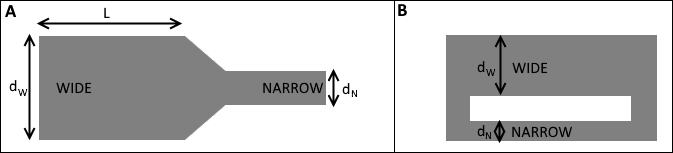
\includegraphics[width=0.8\textwidth]{micro-devices.png}
	\caption{Microfluidic channels in series (A) and in parallel (B).}
	\label{fig:series-parallel}
\end{figure}

Both of the devices consist of two channels connected to each other.
In Device A, the wide and narrow channels are connected in sequence.
In Device B, the wide and narrow channels are next to each other, but both fed from the same inlet and outlet.
In other words, the channels of Device A are in ``Series'' and the channels of Device B are in ``Parallel.''
In these devices, the width, $d$, of the wide channel (6.0 mm) is twice the width of the narrow channel (3.0 mm), and the lengths and depths (not shown in the top view) of the wide and narrow channels on each slide are equivalent.
To drive the fluid through the devices, the video makers used a plunger syringe and applied a force to the plunger that was as steady and repeatable as possible.
\newpage
As the fluid (containing 5 $\mu$m beads) flows from the left side to the right side of the
microfluidic devices, the volumetric flow rate of the fluid, $Q = v*A$, will be governed by the HagenPoiseuille (H-P) equation:
\[ \Delta P \propto \left( \frac{\mu L}{A^{2}} \right) Q \]
where $L$ is the length of the channel, $\mu$ is the viscosity of the fluid, $A$ is the area of the channel ($A = d*depth$), and $\Delta P$ is the change in pressure between the ends of a channel.

\paragraph{For this two week lab:} Your overall task for the next two weeks is to use ImageJ to measure the motion of microbeads as they travel through various microfluidic devices.
\begin{enumerate}
\itemsep-0.2em
\item Qualitatively analyze your videos and use the descriptions of the motion in your report.
\item Make sure that you understand how to use ImageJ to analyze video.
\item Measure the motion of at least ten particles in each of the videos.
\end{enumerate}

\section*{Part 1: Qualitative Analysis}
To start your investigation (\emph{before} you begin analyzing videos), look at the motion of the
beads \emph{both} for the slide of channels in Series (Device A) \emph{and} for the slide of channels in Parallel (Device B).
These videos are on your computer.
For each device:
\begin{itemize}
\itemsep-0.2em
\item is the motion faster in the wide channel or in the narrow channel, and
\item is the pressure drop higher in the narrow or wide channel?
\item Does this pattern match for the two devices? Why or why not?
\end{itemize}
Qualitatively describe what you see and justify/explain why you are seeing what you are seeing using the H-P equation.
Consider what biological systems might be modeled using the Series and Parallel devices.
This portion of the lab may take you 30 minutes or more.
Be thorough!

\section*{Part 2: Quantitative Analysis}
For one of these devices, analyze the videos of the motion of the beads in both the wide and
the narrow channels.
(These videos were collected using a 40x optic and a medium-level resolution (1024 pixels).
The frame rate for each video is in the file name.)
Do a quantitative analysis of these videos using ImageJ and Excel to investigate the relationship between the relative widths, $d$, of the channels and the relative velocities, $v$, of the beads in those channels.
If you are unfamiliar with these tools, read Technical~Documents~\ref{chap:excel-analysis} and \ref{chap:imagej}.
%\par
%Working together with a lab group that analyzed the other device, make sense of your collective data.
%Compare your answers to the questions in the previous paragraph and consider how to answer these questions with respect to the entire data set.
%Professional scientists often make use of data collected and analyzed by their peers in order to further their own investigations.
%What are some of the factors limiting the adaptation and use of data you have not collected for yourself?
\paragraph*{Things you might consider including in your lab report:} In addition to the standard lab report, be sure to include a thorough discussion of both the qualitative and quantitative analyses of the motion of the beads through the microfluidic devices.
For both flow geometries, discuss a possible biological or medical consequence of the H-P equation.
Some other questions you may want to consider:
\begin{itemize}
\item Is the H-P equation a good description of the relationship between $d$ and $v$? Why or why not?
\item What assumptions are you making in our data collection and analysis? What assumptions are you making in comparing your results to the H-P equation? Are these assumptions valid?
\item Do you have enough information to calculate the depth of the channel? If not, what other information would you need to complete the depth calculation? Explain your reasoning.
\end{itemize}
\newpage{\blankpage}
\chapter{Electrophoresis and Charge Screening in Fluids}
\thispagestyle{fancy}
\fancyhead[RE,LO]{Experiment \thechapter}
%
The biophysical motivation for this laboratory is the ubiquity of charges in living systems.
Large molecules—in particular, proteins—are often phosphorylated and thus carry net charge.
These charges generate electric fields, exerting attractive forces on other molecules, and playing a role in the intricate balance of forces and movements that occur in a living cell!
We might ask: how far is the reach of the force field from a charge in a large protein when many ions are present in the surrounding fluid?
How fast would a charged protein move in an electric field?
These effects are crucial for understanding biological systems at the cellular level.
\par 
In this experiment, we will investigate related questions in a simple model system.
You will be investigating charge screening in fluids by employing the technique of electrophoresis.
Your investigation will come in two parts: an investigation of glass beads in de-ionized water (DI water, pure H$_{2}$O), and an investigation of glass beads in two saline solutions of different concentrations.
\par 
%We have been employing solutions of glass beads in water in most of our labs.
You may notice that some of the beads are stuck together, forming clumps (also called `flocs' because their aggregation (coming together) is a form of `flocculation'), or that the beads sometimes ``settle-out'' of the fluid (like the sedimentation we observed in the tilted microscope lab last semester). 
Aggregation (flocculation or coagulation) and sedimentation are behaviors common to colloidal fluids. 
A colloidal system is one in which one phase of matter is finely dispersed throughout another phase of mater. 
Our glass beads in water are colloidal fluids because the glass beads (solids) are small particles dispersed throughout the water (fluid). 
\par 
When the glass beads are submerged in water, they become charged — even in DI water! 
The glass beads, SiO$_{2}$, have surface groups of SiOH. 
When immersed in water, the hydrogen nucleus breaks free (increasing the acidity of the fluid due to the roaming H$^{+}$) and leaving an SiO$^{-}$ behind. 
Thus the surface of the glass beads becomes negatively charged — each bead carries charge on the order of femto-Coulombs (fC). 
(Lest you think a fC is small, about how many extra electrons are on each bead?) 
[You might then ask, if all the beads are negatively charged, then why do they stick together? 
Besides the electric repulsive forces between the beads, there are also attractive van der Waals forces; at close enough distances, the attraction dominates the interaction and the beads will stick together to form a floc.] 
If a salt (like NaCl) is added to the fluid, it will dissolve and the free cations (or anions, for a positively charged colloid) will group around the negatively charged beads of glass, thus decreasing the `effective charge' of the unit — this is called `charge screening' or `Debye screening.' 
The more ions that are available in the fluid, the greater the charge screening effect will be; thus the concentration of the electrolyte is important.
\par 
We can investigate these charges using the technique of electrophoresis. 
By applying an electric field (generated by a potential difference between two electrodes) to the fluid, we can cause an electric force on the charged beads that will induce motion through the still fluid.
A larger electric field will cause faster motion. 

\paragraph{For this two week lab:} Your overall task for the next two weeks is to determine how charged our glass beads are in DI water and then compare that charge to the `effective charge' as seen in various concentrations of saline solution.
You will do this in multiple stages:
\begin{enumerate}
\itemsep-0.2em
\item Create a model of the forces acting on your beads in a solution.
\item Discuss as a class what you need to measure, and how you will calculate the charge on your beads.
\item Capture your first video according to table~\ref{tab:lab7-vids} and analyze it. Make sure that the surface charge values that you calculate make sense.
\item Collect the rest of your videos and analyze them.
\end{enumerate}

\section{Modeling Electrophoresis}
Before you begin taking data, you will need to model the situation: consider what forces act on the bead as it moves through the fluid and determine how changing the potential difference between the electrodes and measuring the resultant speed of the beads will enable you to find the charge on the beads. 
Carefully reflect on what assumptions you are making as you model the situation and think about the implications these assumptions have for the design of your experiment.
\par 
After modeling the situation, design an experiment to determine the charging of beads in fluid. 
Consider 'broad stroke' details (e.g., What data are we collecting? How much data is 'enough'?) as well as 'fine stroke' details (e.g., What part of the slide are we viewing? How are we collecting data? How do our assumptions affect our procedure and analysis?). 
Be sure to consider the qualitative aspects of the motion, as well (e.g., Is this really directed motion? Could it be random motion? Which electrode (+ or -) are the beads moving toward?). 
Once you have a good experimental design, gather data to determine the charging of our glass beads in DI water.

\section{Measuring Electrophoresis}
For this experiment, you will be using a microscope to observe the motion of aqueous micropheres within an electric filed. If you are unfamiliar with how to operate a microscope, including how to capture video using one, please read through Technical~Document~\ref{chap:scope-basic}. The experimental set-up available includes:
\begin{itemize}
\itemsep-0.3em
\item Microscope with camera.
\item Power source to create constant voltage of your choosing
\item Two wires with banana plugs on one end and alligator clips on the other (for holding electrodes, see figure~\ref{fig:electroph})
\item Short segments of copper wire to use as electrodes
\item A 24 well plate (fill one of these chambers with enough solution to cover the bottom for each investigation — when investigating a different solution, you can simply move to another chamber. At the end of the the first day, please put your name on your chamber slide and store in the cabinet. Each well has a diameter of 15.5 mm.)
\item Three vials of solution: one of distilled water and two different saline solutions (LOW and HIGH)
\item Other tools (rulers, paper towels, pipettes, etc.)
\end{itemize}

\noindent
If you have never used a power source before, ask your TA for safety and use instructions. Here are some other details that may help you while performing your experiment:

\begin{itemize}
\itemsep-0.3em
\item The maximum voltage the power source can produce is 18 V; you will likely need 4 V or more to see bead motion in DI water.
\item The wells each need less than 1 mL of fluid to coat the bottom; the vials provided should be sufficient.
\item You should gather your video data as soon after applying the potential difference to the
electrodes as possible.
\item You should be careful to leave the fluid sample on the microscope stage (above the hot
bulb) for as short a time as possible before gathering your video (think about why this might
be so).
\item Be sure to note the timing used by the video capture program for each video taken.
\end{itemize}

\begin{figure}[hbtp]
	\centering
	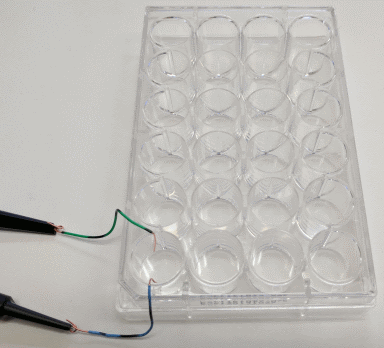
\includegraphics[scale=0.70]{electrophoresis}
	\caption{Electrode setup for investigating electrophoresis.}
	\label{fig:electroph}
\end{figure}

Now investigate how saline solutions 'screen' the charge on the glass beads, by determining their `effective' charge in the various solutions that you are asked to investigate in table~\ref{tab:lab7-vids}.

\begin{table}[ht]
	\centering
	\begin{tabular}{|c|c|c|}
	\hline 
	\textbf{Group} & \textbf{Video 1} & \textbf{Video 2} \\ 
	\hline 
	1 \& 2 & 2 um beads in DI & 2 um beads in LOW \\ 
	\hline 
	3 \& 4 & 2 um beads in DI & 2 um beads in HIGH \\ 
	\hline 
	5 \& 6 & 5 um beads in DI & 5 um beads in LOW \\ 
	\hline 
	\end{tabular}
	\caption{Videos. `DI' refers to De-Ionized water. `LOW' refers to a saline solution with 9 mg/L NaCl; `HIGH' refers to a saline solution with 90 mg/L NaCl. The viscosities of these solutions are almost identical: $9.0 \times 10^{-4}$ Pa s at 26 $^{\circ}$C.}
	\label{tab:lab7-vids}
\end{table} 

\paragraph*{Things you might consider including in your lab report:} In addition to the standard lab report, be sure to include a thorough discussion of both the qualitative and quantitative differences between the two solutions that you investigated.
Also discuss how you modeled the situation, how your model informed which forces you needed to consider, and what equation did it lead you to derive to calculate the charge of the glass beads in the fluid.
Discuss the ways in which the ideas explored here relate to biology and/or chemistry.
%Some other questions you may want to consider:
%\begin{itemize}
%\item 
%\item 
%\item 
%\end{itemize}
%\newpage{\blankpage}
\chapter{Testing Models of Signal Transmission Along Nerve Axons}
\thispagestyle{fancy}
\fancyhead[RE,LO]{Experiment \thechapter}

\begin{wrapfigure}{r}{0.45\textwidth}
  \vspace{-25pt}  
  \begin{center}
  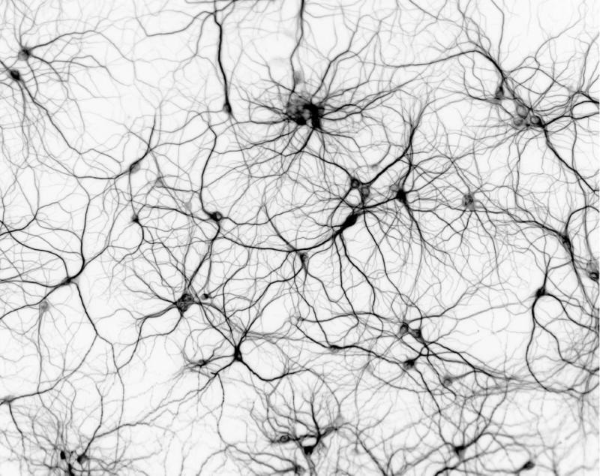
\includegraphics[width=0.43\textwidth]{neural_nets}
  \end{center}
  \caption{Neurons form networks for information flow.}
  \label{fig:neural_net}
  \vspace{45pt}
  \begin{center}
  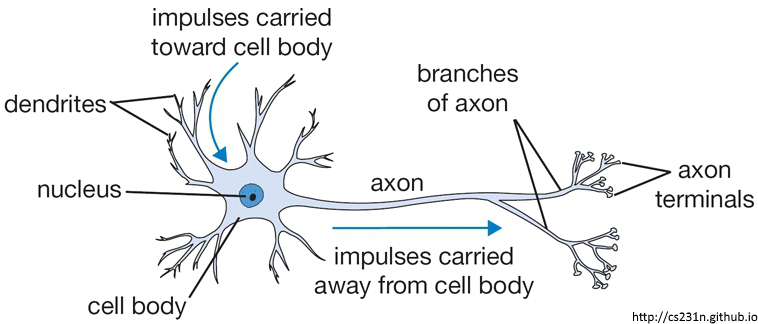
\includegraphics[width=0.43\textwidth]{neuron2}
  \end{center}
  \caption{Information flow through neurons.}
  \label{fig:neuron}
  \vspace{0pt}
\end{wrapfigure}

Nerve impulses travel in our bodies as electrical signals. 
Whether its seeing or hearing something, controlling a muscle, or just thinking, the transmission process along a nerve cell, or neuron, is the same: a sufficient stimulus received by the cell body (\emph{soma}) initiates a change in the potential difference across the membrane, or \emph{action potential}, which travels along the axon to be transferred through a synapse to the other neurons or muscle cells. 
[See figures~\ref{fig:neural_net} and \ref{fig:neuron}]
A single axon can be a meter or more long, like those connecting our toes to our spinal cords, so action potentials must travel a long way.
You may have learned in a biology course that for an action potential to be transmitted from one end of an axon to another, it must be regenerated repeatedly along its length.
We call this \emph{active transport} and it is accomplished by voltage-gated ion channels, as discussed in the appendix to this lab.
Why is active transport necessary?
Couldn't we simply apply a potential difference to the end of a nerve axon and expect that signal to travel along the axon to its final destination, the spinal cord and then the brain?
This alternate type of signal transmission is called \emph{passive transport}. 
In this two week lab sequence, we will be \textbf{modeling passive transport} in nerve axons and \textbf{testing our model} to determine if passive transport is a feasible method of signal transmission. 
We will also be \textbf{considering some adaptations} to the simple cylinder model of a nerve axon that can increase the speed of signal transfer – surely a faster response is advantageous to survival in a species!

\subsection*{Simple cylinder model of a nerve axon: structure and properties}

%\begin{wrapfigure}{R}{0.45\textwidth}
%  \vspace{-25pt}  
%  \begin{center}
%    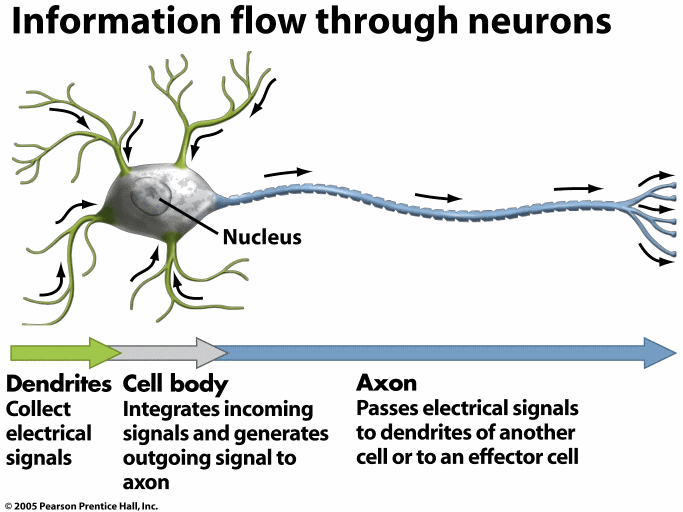
\includegraphics[width=0.43\textwidth]{neuron}
%  \end{center}
%  \caption{Inside a cell wall.}
%  \label{fig:neuron}
%  \vspace{-5pt}
%\end{wrapfigure}

The structure of the axon is shown schematically in figure~\ref{fig:axMod1} below.
For electrical purposes, an axon is basically a long, thin cylinder of membrane filled with a fluid called axoplasm.
When no action potential is traveling, the potential difference across the membrane, from the outside of the axon to the inside, is about -70 mV, the \emph{resting} potential difference.
In part, this is because the concentration of of sodium atoms (Na$^{+}$) is much higher outside the axon than inside.
\par
The axoplasm, like all fluids in biological systems, has mobile ions dissolved in it, giving it a moderate conductivity (many orders of magnitude lower than copper or other metals we can think of as ideal conductors).
The fluid outside the membrane, the \emph{extracellular fluid}, is very similar to the axoplasm and thus has approximately the same conductivity.
\par 
The lipid bilayer forming the membrane is electrically insulating, with extremely low conductivity, but many different kinds of channel proteins cross the membrane.
These channels only allow specific ions to pass under particular conditions,
The channels increase the conductivity of the membrane as a whole, so that although the membrane conductivity is much lower than that of the axoplasm, current \textbf{does pass} through the membrane.

\begin{figure}[hbtp]
	\centering
	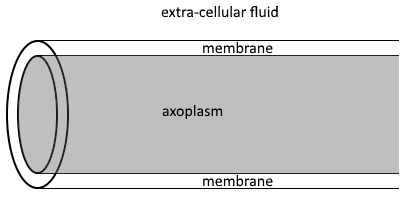
\includegraphics[width=0.4\textwidth]{axonModel1}
	\caption{Simple cylinder model of an axon.}
	\label{fig:axMod1}
\end{figure}

\section*{Part 1: Modeling Passive Transport}
Our goal is to understand how a potential difference applied across the membrane at one end of the axon spreads along the axon if it is not being regenerated as it travels down the axon.
thus for the purposes of our model we'll assume there is a battery at the left end of the axon segment (see figure~\ref{fig:axMod2}), holding the potential difference from the outside to the inside at $x=0$ to a positive value we'll call $V_{0}$.

\begin{wrapfigure}{R}{0.45\textwidth}
  \vspace{-25pt}  
  \begin{center}
    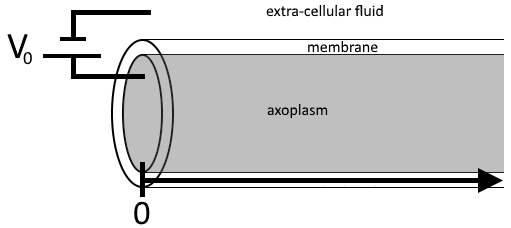
\includegraphics[width=0.43\textwidth]{axonModel2}
  \end{center}
  \caption{Model of potential difference across axon membrane.}
  \label{fig:axMod2}
  \vspace{-5pt}
\end{wrapfigure}

\par 
Suppose there was just a single ion channel (e.g., a `potassium leak channel') crossing through the membrane, at the right end of the segemnt in the figure. 
\textbf{Draw a loop} onto the diagram showing the path of current flow from the positive side of the battery (inside) to the negative side of the battery (outside), and then \textbf{draw a simple circuit} that corresponds to this pattern of current flow.
(You may want to include this in the introduction of your lab report)
The axoplasm, an ion channel, and the extracellular fluid should each be represented separately in your simple circuit.
\par 
In fact, the resistance of the current path through the extracellular is much less than the resistance of either the axoplasm or the ion channel through the membrane, so the extracellular fluid can be represented as just a conducting wire in the simple circuit.
(If you didn't initially do so, update your simple circuit accordingly.) 
Let's think about why the extracellular fluid will have such low resistance.
\par 
Resistance $R$ can be determined from the length $L$, the cross-sectional area $A$, and the resistivity $\rho$ according to $R = \frac{\rho L}{A}$.
The resistivities of the axoplasm and the extracellular fluid are very similar.
Considering how the current flows through both the axoplasm and the extracellular fluid, \textbf{explain why} the resistance of the current path through the extracellular fluid is much smaller than the resistance of the current path through the exoplasm - thus we can treat the extracellular fluid as just a conducting wire.
\par 
A long axon can be modeled as a chain of many short segments like the segments like the segment described above.
The dashed lines in figure~\ref{fig:axMod3} visually divide the axon into five such segments.
Sketch the path of current flow onto the diagram and then \textbf{design a circuit model} for it.
\textbf{Check your model with your instructor.}
\par 

\begin{wrapfigure}{R}{0.45\textwidth}
  \vspace{-15pt}  
  \begin{center}
    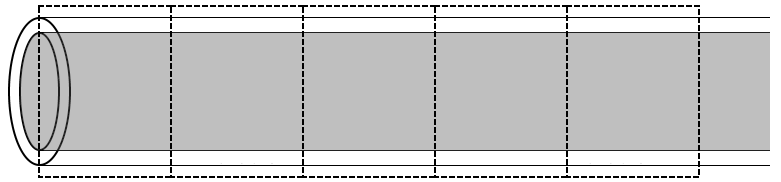
\includegraphics[width=0.43\textwidth]{axonModel3}
  \end{center}
  \caption{Axon chain of many segments.}
  \label{fig:axMod3}
  \vspace{-5pt}
\end{wrapfigure}

To complete the model, we need values for the resistances.
There are actually many ion channels passing through the membrane, so our circuit model needs to be constructed using the resistance of a segment of membrane rather  than a single ion channel.
Each segment of membrane consists of many ion channels in parallel, so the overall resistance of the membrane segment is the equivalent resistance of all of those ion channels. 
The average resistivity of the membrane can be measured and used to find the resistance of a segment of membrane.
\par 
Use the relationship between resistance, resistivity, length, and cross-sectional area to \textbf{estimate values for the resistance} of a membrane segment $R_{mem}$ and an axoplasm segment $R_{axon}$ using the following order-of-magnitude values:
\begin{itemize}
\itemsep-0.2em
\item the diameter of the axon $\sim$ 10 $\mu$m
\item the membrane thickness $\sim$ 10 nm
\item the resistivity of the axoplasm $\sim$ 1 $\Omega$-m
\item the average resistivity of the membrane $\sim  10^{8} \; \Omega$-m
\item the segment length $\sim$ 1 mm
\end{itemize}
Hint: To determine the cross-sectional area of a membrane segment, think of unrolling the membrane from the axon.
Also, it turns out that only the ratio $R_{mem}/R_{axon}$ affects how far the potential difference will spread.

\section*{Part 2: Qualitative Analysis of Your Model}
With the model you have created, we hope to understand how the potential difference across the membrane changes as we examine different distance along the nerve axon.
In other words, how is the voltage across the membrane at a distance $x$ related to the initial voltage $V_{0}$?
Before we collect data and perform a quantitative analysis of your model, let us \textbf{think qualitatively about some of the features of your model of passive transport}.
\par 
We want to understand how the voltage across the membrane depends on the distance along the axon.
Each segment in you multi-segment model circuit should include a resistor representing the membrane, so the voltages across these resistors represents $V_{mem}$ at each segment.
The first $R_{mem}$ corresponds to segment 1, the second to segment 2, and so on. 
Let's notate these voltages as $V_{mem}^{1}$, $V_{mem}^{2}$, and so on.
Similarly, let's call the voltages across the axon segments $V_{axon}^{1}$, $V_{axon}^{2}$, and so on; the currents in the axon segments are $I_{axon}^{1}$, $I_{axon}^{2}$, and so on.
\par 
\textbf{Applying the loop rule} to the first segment, find in terms of the applied membrane potential $V_{0}$, the current in the first axon segment $I_{axon}^{1}$, and the membrane resistance $R_{axon}$.
Do the same for the second segment, finding $V_{mem}^{2}$ in terms of the applied membrane potential $V_{0}$, the axon currents, and the resistance $R_{axon}$.
\emph{Is $V_{mem}^{2}$ less than, equal to, or greater than $V_{mem}^{1}$? How do you know?}
Do the same for the third segment, finding $V_{mem}^{3}$ in terms of the applied membrane potential, the currents in the segment, and the axon resistance.
With $n$ indicating the segment number, does $V_{mem}^{n}$ increase or decrease as $n$ increases?
Does $I_{axon}^{n}$ increase or decrease as $n$ increases? 
On your circuit diagram, draw arrows of different widths (or lengths) by each axon resistor to indicate the amount of current in the axon segment.
\par 
From your analysis, it should be clear that $V_{mem}$ decreases as you go further and further from the start of the axon.
Can we be more specific?
If we create a mathematical model for $V_{mem}(x)$ as a function of $x$, where x is the distance from the start of the axon, what functional form would we expect?
As a reminder, common possibilities include:
\begin{enumerate}
\itemsep-0.2em
\item linear with a negative slope (rate of change is constant)
\item inverse (product is constant)
\item exponential decay (percent change is constant)
\end{enumerate}
It should help to consider the behavior of $V_{mem}(x)$ in the limiting cases.
Examine the behavior of your model circuit.
As $x$ approaches $0$, what happens to $V_{mem}(x)$?
As $x$ becomes very large, what happens to $V_{mem}(x)$?
Compare with the behavior of each of the possible functional forms.
Make your best guess for the functional form and sketch the corresponding graph of $V_{mem}(x)$ vs. $x$.
Explain your reasoning.

\section*{Part 3: Quantitative Analysis of Your Model}
You are now ready to build and test your passive transport circuit model.
\par 
Equipment:
\begin{itemize}
	\itemsep-0.2em
	\item circuit board
	\item connecting wires
	\item alligator clips
	\item battery 
	\item switch
	\item assorted resistors
	\item voltage probe
	\item LabPro
	\item computer and LoggerPro software
\end{itemize}
The circuit board (also known as a ``breadboard'') is probably new to you and requires a short explanation (see figure~\ref{fig:breadboard}).
Down the edges of the board are two columns of holes surrounded by a red and a blue line.
Leave the negative end of the battery connected to the blue line; this is your extracellular fluid and all of these holes are connected together in this column (connected inside the circuit board).
The other parts of the circuit board are much wider sets of columns.
For these, the holes in a column are NOT connected, but the holes in a row ARE connected.
If this is not clear enough for you, please ask your TA to explain.
You will need to think carefully about how you can fit your model of passive transport in a nerve axon onto this circuit board.
You have two circuit boards so that you can begin building a second model with spare resistors once you are ready to test the first model.
\par 

\begin{figure}[hbtp]
	\centering
	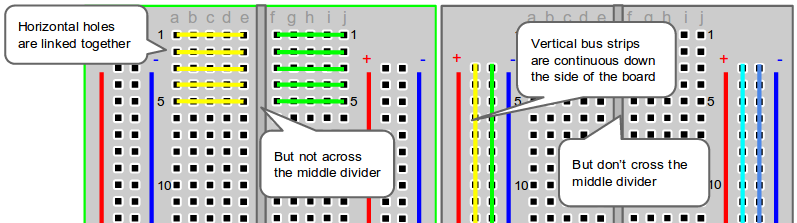
\includegraphics[width=\linewidth]{breadboard-connect.png}
	\caption{Breadboard connections diagram.}
	\label{fig:breadboard}
\end{figure}

\textbf{Construct your model circuit with ten segments} using the provided components.
Choose resistors with the proper ratio of resistance values that you found in the previous part, and make sure that you use the same value value of resistance for all of the $R_{mem}$ and a different constant value for all of the $R_{axon}$.
Don't forget to close the switch to take data and open it when you finish.
\par 
\textbf{Measure and record} $V_{mem}$ vs. $x$ for $x = 0 \, mm$ to $x = 10 \, mm$.
(In your circuit, each axon resistor corresponds to a 1 mm segment, so for your measurements, x is the segment number.
At $x=0$, $V_{mem}(x)=V_{0}$.)
To record voltages in LoggerPro:
\begin{itemize}
\itemsep-0.2em
\item Click on the Data Collection icon, and change the mode to ``Events with Entry.'' Provide appropriate name and units. Click `Done'.
\item Press the start button.
\item Use the voltage probe to measure voltages by attaching the probe leads to the circuit on either side of each $R_{mem}$. To store voltage values in a table, click on `Keep Current Value'. You can enter the corresponding length value in the same row of the table. Don't forget to collect the $x=0$ value $V_{0}$!
\item If a Data Erase box appears, click on `Append to Latest Data' and proceed.
\item Press the stop button when finished with all 11 data points.
\item To display data points without connecting lines, double click on the graphed data, and unselect the option for connecting the data points.
\end{itemize}
Now let's \textbf{interpret your results}.
Following the same line of reasoning you used in your qualitative analysis to find $V_{mem}^{n}$, and assuming that the segment is only a different length $dx$ long, it is possible to derive a differential equation for $V_{mem}(x)$ - don't do this, just know that it is possible!
Solving the differential equation gives us an equation describing how the voltage across the membrane depends on the distance $x$ from the end where a voltage $V_{0}$ is applied.
The equation is then:
\[ V_{mem}(x) = V_{0} e^{-x/\lambda} \quad \textrm{with} \quad \lambda =\alpha \sqrt{\frac{R_{mem}}{R_{axon}}}  \]
where $\lambda$ (Greek letter lambda, called the length constant of the axon) is the distance along the axon at which $V_{mem}(x)$ has decreased by a factor of $e$ (the natural logarithm base e), to $0.37 V_{0}$, and $\alpha$ is a proportionality constant with units of length that is specific to different types of axons.
\par 
To perform a fit:
\begin{itemize}
\itemsep-0.2em
\item Click `Analyze'.
\item From the drop-down menu select `curve fit'.
\item From the pop-up menu select the appropriate function for exponential decay.
\item Click `Try Fit'.
\item If it is the correct fit click `Ok'.
\end{itemize}
Provide the graph of your data with your best fit function in your lab write-up.
Calculate the length constant of your model circuit from your best fit function.
What does this length constant tell you about the feasibility of passive transport as a signal transmission method?
Will your brain ever be informed of an injury to your toe?
Given the length constant you have determined, how many `lengths' are there in the nerve connecting your toe to the base of your spine?
What fraction of the original potential difference ($V_{0}$ at your toe) remains by the time the signal reaches the spine?
\par 
Build two new model circuits with two different length constants and find these length constants with a few measurements (you don't have to measure as many data points if you choose them wisely; include the graphs for these two circuits in your report).
How does the length constant change as the ratio of $R_{mem}$ to $R_{axon}$ changes?
To get a signal from your toe to reach the base of your spine using passive transport, \textbf{what would the ratio of the resistance need to be}?
State your assumptions.

\newpage

\section*{Part 4: What adaptations allows the action potential to travel faster?}
How fast does an action potential travel along an axon?
You're probably aware that it's finite - no one has truly instant reflexes.
Yet, your model circuit suggests that the process is nearly instantaneous.
Something is missing from the model.
We need to extend our model in order to understand \emph{why} it takes time for an action potential to travel along an axon.
\par 
Let's take a closer look at the membrane of an axon.
[See figure~\ref{fig:memRC}A below.]
The channels are the paths through which ions flow (with some resistance).
The equivalent resistance of all of these parallel channels in a single segment is $R_{mem}$.
Now take away those channels and what do you have left?
An insulating layer with conducting fluids on each side.
That should remind you of a familiar device - a capacitor.
The membrane is therefore properly viewed as a resistor and a capacitor in parallel.
[See figure~\ref{fig:memRC}B below.]
As current travels along the axon and enters each new segment, charge also accumulates on the capacitor.
It takes a significant amount of time for a capacitor to charge and thus also for the potential difference across the membrane to reach its final destination.
We refer to the time it takes the membrane potential difference to reach 63\% of its final value as the time constant $\tau$.
It can be shown that $\tau = R_{mem}C_{mem}$, where $R_{mem}$ is the resistance and $C_{mem}$ is the capacitance of a segment of membrane.
It takes several time constants for the membrane potential difference to reach the values that your model resistor circuit gives.
\begin{figure}[hbtp]
\centering
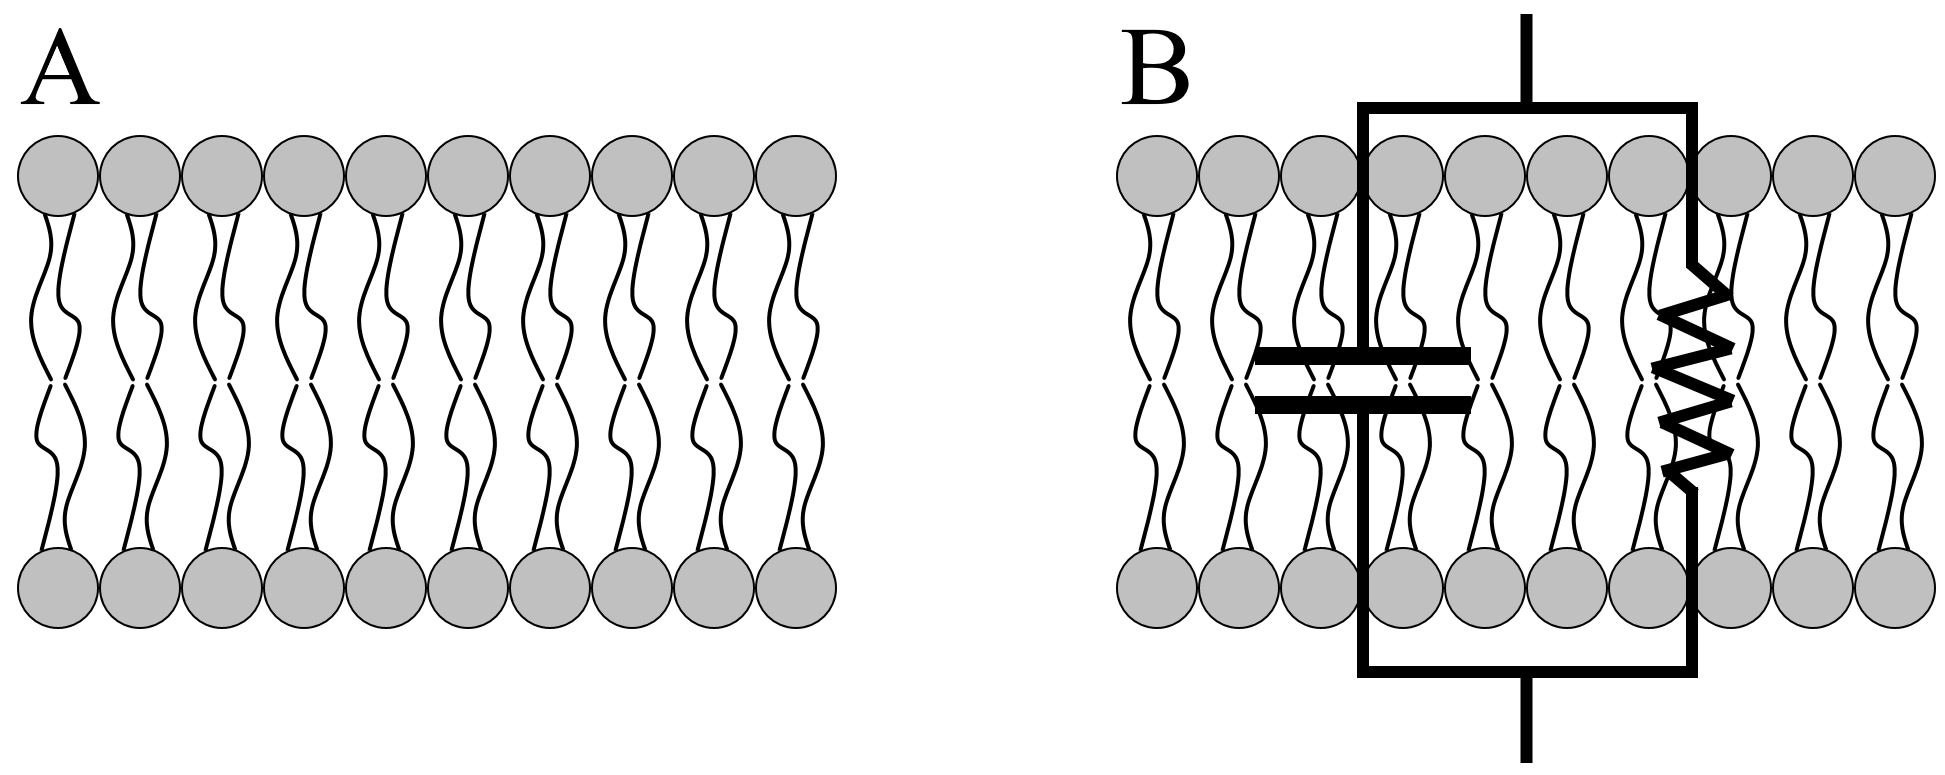
\includegraphics[width=0.5\textwidth]{membraneRC}
\caption{(A) magnified view of a membrane. (B) RC circuit model of a membrane.}
\label{fig:memRC}
\end{figure}


\subsection*{Speed depends on time constant and length constant}
The speed at which an action potential travels down an axon depends primarily on two things:
\begin{itemize}
\itemsep-0.2em
\item \textbf{It's \emph{inversely proportional} to the time constant:} The longer it takes the membrane potential difference to rise in each segment, the slower the action potential will travel. The time constant is given by $\tau = R_{mem}C_{mem}$.
\item \textbf{It's \emph{proportional} to the length constant:} The greater the length constant, the farther the depolarizing potential difference reaches down the axon without regeneration, bringing successive segments to the threshold potential difference required to regenerate the action potential sooner. You measured the length constant of your model circuit in Part 3. In general, the length constant $\lambda$ is proportional to $\sqrt{R_{mem}/R_{axon}}$. This makes sense: If the membrane resistance is really big (or if the axon resistance is really small), current mostly flows \emph{down} the axon, with just a little flowing across the membrane in each successive segment.
\end{itemize}
It makes sense that faster propagation of nerve impulses confers an advantage to an organism.
In the next few questions, we'll \textbf{examine the physics behind some adaptations leading to speedier action potentials}.

\begin{figure}[hbtp]
	\centering
	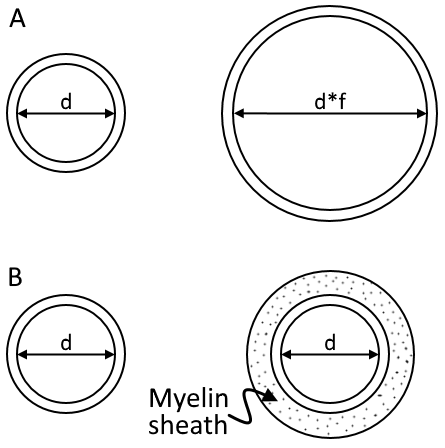
\includegraphics[width=0.5\linewidth]{axon_alt}
	\caption{caption}
	\label{fig:axon_alt}
	\vspace{-20pt}
\end{figure}

\subsection*{How does making the axon wider affect the speed?}
Let's say the diameter of the axon is increased by a factor of $f$. [Figure~\ref{fig:axon_alt}A]
\begin{enumerate}
\itemsep-0.2em
\item By what factor does $R_{axon}$ change? (Note: The resistivity of the axoplasm is constant, as is the 1 mm length of an axon segment.)
\item By what factor does $R_{mem}$ change? (Note: The resistivity of the membrane is constant, as is the 1 nm thickness of the membrane.)
\item By what factor does the length constant $\lambda$ change?
\item Assuming that the time constant doesn't change, by what factor does the speed therefore change?
\item By what factor would the diameter of the axon have to change to increase the speed by a factor of 10?
\end{enumerate}
Note: The `wider axon adaptation' is the strategy adopted by the squid, whose `giant' axons allow very rapid travel of its action potentials, making it a master of the quick escape.

\newpage

\subsection*{What about making the membrane thicker?}
Wider axons work fine for a squid, but are highly impractical for organisms with lots of neurons like humans.
(If each of your neurons were the size of a squid's, your head wouldn't fit through a doorway!)
Let's explore another possible way of increasing the length constant and therefore the speed: increasing $R_{mem}$.
This is a strategy commonly adopted by vertebrates.
It's achieved by extra insulation (a myelin sheath) that's wrapped around the axon. [Figure~\ref{fig:axon_alt}B]
\begin{enumerate}
\itemsep-0.2em
\item Let's say that myelination increases the membrane resistance by a factor of 1000. By what factor does the length constant increase? Why?
\item Assuming that the time constant doesn't change, by what factor do the speed therefore change? Why?
\item Based on the analysis you did in part 3, could a myelinated axon use passive transport as the signal transmission method? Why or why not?
\item There are many diseases that affect signal transmission along neural pathways. These include multiple sclerosis (MS), myasthenia gravis, and amyotrophic lateral sclerosis (ALS or `Lou Gehrig's Disease'). Often, a component of these afflictions is a malformation or degeneration of the myelin sheath. MS is a demyelinating disease, which means that the axons of neurons are intact but the myelin sheaths are damaged. Why would loss or damage to the myelin sheath be a problem for signal transmission, even if the axon was intact?
\end{enumerate}
Note: Myelination obstructs the membrane's voltage-gated Na$^{+}$ channels that enable the action potential to be regenerated.
For this reason, there are gaps in the myelin coating, called the nodes of Ranvier, where the channels are not obstructed.
From what you've learned in this lab, what do you suppose determines the maximum distance between these gaps?

\section*{For your report:}
As stated previously, the \textbf{lab write-up} should include (a) your explanations of the models you made, (b) the supported conclusions you drew from analyses of your models, and (c) your discussion of advanced topics related to the basic ideas yoiu are exploring.
To be more specific, you should discuss the work you have done and the considerations you have made in modeling passive transport, qualitatively and quantitatively analyzing your model, and modeling adaptations that can increase the speed of signal transfer.
If you want to include hand-drawn elements (such as model circuit diagrams), please do so.
Don't forget to include the plots of $V_{mem}(x)$ vs. $x$ with the appropriate fitting functions. 
\underline{Respond explicitly} to all passages marked with an exclamation point (!).

\newpage{\blankpage}
\chapter{Exploring Light and Lenses}
\thispagestyle{fancy}
\fancyhead[RE,LO]{Experiment \thechapter}
%
Optics — the sub-field of physics focusing on the study of light — is important to many areas of biology, including vision, ecology, botany, neurobiology and molecular biology. 
The use of optics in biology has evolved from the simple light microscope used by Darwin to the complex, live-cell, high resolution microscopes used in current cutting-edge research. 
In this two-week lab, we will be exploring the behavior of light and lenses. 
Microscopes usually employ at least two lenses together—but, as we are only beginning to learn about light, we will be exploring single-lens systems. 
\par 
%Your task is two-fold: 1) Design a way of determining the focal lengths, f, for five converging (bi-convex) lenses; and then, 2) Design an experiment to explore how the focal length, f, of a lens interacts with the image distance, i, and object distance, o, when the total distance, from object to image, is a fixed length, L. 
\begin{figure}[hbtp]
\centering
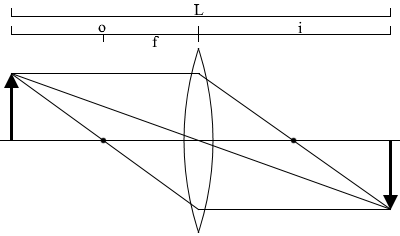
\includegraphics[width=0.5\textwidth]{lensDiagram}
\caption{Ray diagram of a single-lens system.}
\label{fig:lensDiagram}
\end{figure}

A typical single-lens system is shown in figure~\ref{fig:lensDiagram}. The image distance, $i$, is the distance from the location of the image to the center of the lens. 
The object distance, $o$, is the distance from the location of the object to the center of the lens. 
For most microscopes, the object location and image location cannot be changed (they are a fixed distance, $L$ apart), so it is the type of lens (and thus its focal length, $f$) and the location of the lens that are changed to achieve different magnifications and to focus the image. 
Ultimately, you should be able to construct a mathematical model of the interaction of focal length and image/object distance that is supported by your data. 
Think carefully about your experimental designs and how they affect your sources (and values!) of uncertainty.

\paragraph{For this two week lab:} Your overall task for the next two weeks is to design a way of determining the focal lengths for five converging (bi-convex) lenses.
Then, design an experiment to explore how the focal length of a lens interacts with the image distance and object distance when the total distance from object to image is a fixed length.
You will do this in multiple stages:
\begin{enumerate}
\itemsep-0.2em
\item Get familiar with the optical equipment. Make sure that the lenses are clean, if they are not, ask your TA for help cleaning them.
\item Determine the focal lengths of your lenses.
\item Explore how the focal length of a lens interacts with the image distance and object distance when the total length from object to image is fixed.
\end{enumerate}

\section*{About the Equipment:}
Each group has access to:
\begin{itemize}
\itemsep-0.3em
\item a light source (your object)
\item five converging (bi-convex) lenses of differing focal lengths
% \item one diverging (bi-concave) lens
% \item a lens holder with pole clamp
\item a long optical rail
% \item small LED light boxes emitting different colors of light,
% \item a light box with a plano-convex lens,
\item a meter stick and a ruler, and
% \item a simple light microscope à la Darwin.
\end{itemize}
Be sure that your optical elements, such as lenses, are carefully aligned with the vertical axis of your equipment. 
If you need help with this, or are not sure why this is important, please ask your TA. 
Additionally, please be gentle with the equipment, especially the glass lenses, and try to avoid getting finger-prints, skin oils, or dirt on the lenses.
\paragraph*{Things to consider including in your lab report:} In your lab write-up, you may want to include careful discussions of:
\begin{itemize}
\itemsep-0.3em
\item your methods for finding the focal lengths and investigating the $f/i/o$ relationships
\item your data and your analysis of the data
\item your mathematical model for the interaction of focal length and image/object distances
\item your comparison of your work with the work of other groups, as well as your critique of your experiment and conclusions. 
\end{itemize}
You may also want to include hand-drawn elements (such as ray diagrams).
%\newpage{\blankpage}
\chapter{Spectroscopy - Exploring Emission \& Absorption}
\thispagestyle{fancy}
\fancyhead[RE,LO]{Experiment \thechapter}
%
In this two-week lab, we will be exploring the interaction of light with matter. 
Using spectroscopy (also called spectral analysis, spectrometry, or spectrophotometry), we will examine emission and absorption of light by various substances. 
Spectroscopes (also called spectrometers and spectrophotometers) are measurement tools designed to distinguish different colors of light. 
The spectrometers we will use in this lab detect the intensity of the light (the power-per-area associated with the light) as a function of the wavelength of the light. 
These spectrometers have a sensitivity range from 350 nm to 1000 nm, with a spectral resolution of 2 nm. 
In contrast, the human eye has a sensitivity range from approximately 400 nm (violet) to 700 nm (red), with a spectral resolution ranging from 1 nm (in the green to yellow range) to 10 nm (in the violet and red ranges). 
You may have been exposed to spectroscopy data through your previous chemistry and biology courses. 
To thoroughly understand data, one must know where it came from, its limitations, and its interpretations and potential meanings. 
With this lab we hope to deepen your comprehension of the function of spectrometers and thereby enrich your understanding of the data they produce. 
This will lay a firm foundation for your use of spectroscopy in your broader scientific career. 
\par
Matter has rich internal activity. 
Since matter is bound together in stable situations by forces, it has lots of natural ways to oscillate and resonate. 
The methyl groups on organic molecules can spin around. 
Similarly, long molecular chains can vibrate back-and-forth like a spring. 
Within each atom, electrons are constantly shifting towards and away from the nucleus. 
Each of these processes has a particular wavelength (color) of light associated with it: a specifically-sized photon energy packet is emitted or absorbed. 
Since light can only be absorbed or emitted in these packets, the way different colors of light interact with matter tells us about the energy spacing between the allowed excitation states of atoms and molecules. 
Doing a spectral analysis of light emitted or absorbed by something can give us a lot of information about it. 
Stokes (famous for his study of viscosity) was the first to show that hemoglobin was the molecule responsible for carrying oxygen in the blood—he did this using spectral analysis! 
On an entirely different physical scale, it's spectral analysis that permits us to figure out the composition of stars. 
\par 
Your lab will consist of three parts: I) exploring the quantized atom; II) exploring emission and absorption; and III) considering the evolutionary adaptation of the visible spectrum of the human eye. 
The lab report you turn in at the end of the second week should discuss answers to questions posed in the sections below as well as any insights you gain from your explorations and investigations, along with the data supporting those insights.

\section*{About the Equipment:}
Each group has access to:
\begin{itemize}
\item a spectrometer and fiber optic cable that can interface with the computer via the USB,
\item Logger Pro software for the computer,
\item a small stand with multiple 90-clamps,
\item a long pole with table clamp,
\item an assortment of filters/cards, including Green, Red, Yellow, and UV filters and a diffraction grating,
\item a variety of hand-held diffraction grating spectrometers,
\item a classroom set of light sources/lamps: H, Na, Hg, and UV,
\item small LED light boxes emitting different colors of light (Red, Green, and Blue),
\item a light ray box (with an incandescent bulb that acts as a white light source),
\item a meter stick, and
\item an aquarium (fish tank) that can be filled with water.
\end{itemize}
BE GENTLE WITH THE EQUIPMENT!! 
Handle all heavy equipment with care. 
Watch out for all of the wires and cables. 
Keep all fluids away from the computer and spectrometer.
You may be operating in low light conditions, so proceed with caution. 
The Na and Hg lamps will need to warm-up before they produce a usable spectrum. 
Masking the light ray box will help reduce glare from reflections (ask your TA/LA for help with this). 
You may find it helpful to use the fiber optic sensor in conjunction with a fixed holder/mount.

\section*{A Short Introduction to Light/Quantization:}
The range of all possible light waves is referred to as the Electromagnetic (EM) Spectrum (see figure at right). 
Of this range, the 'visible' portion (sensed by the human eye, ~ 400nm - 700nm) is only a very small section. 
These waves move at a speed of c = 3.0·108 m/s in a vacuum. 
Their frequency, f, and wavelength, $\lambda$, are related with their speed, v, according to: v = f$\lambda$. 
The energy, E, carried by these waves is proportional to their frequency: E=hf, where the proportionality constant, h, is Planck's constant (h = 6.63·10-34 kg·m2/s). 
\par
All of these different waves are produced by electric charges moving, oscillating, and resonating in very specific ways. 
For each resonant frequency producing a photon of light there is an associated packet of energy, called a quantum. 
Because all light is made of these packets, these quanta, we say that light is quantized.

\section*{Part I: Exploring the Quantized Atom}
Perhaps the most 'illuminating' model of the quantization of light is the Bohr model of the hydrogen (H) atom. 
In this model, the proton nucleus of the hydrogen atom is orbited by the single electron at fixed orbital radii. 
When the atom is excited (absorbs energy), the electron transitions from the ground state (lowest energy level) to an excited state. 
The electron will then transition back to a lower energy state, emitting this energy difference between levels as a photon of light. 
The Bohr model is a good model for explaining why only certain frequencies/wavelengths of light are absorbed or emitted by an atom. 
It also explains the Rydberg formula for the emission lines of the hydrogen spectrum—this formula was well-established experimentally as early as 1888, but had no theoretical explanation until the Bohr model was introduced in 1913 (25 years later!). 
Some of the energy level transitions within the hydrogen atom have been given specific names. 
All transitions to/from the ground state (lowest energy level, n = 1) are part of the Lyman series. 
All transitions to/from the 1st excited stated (n = 2) are part of the Balmer series. 
All transitions to/from the 2nd excited state (n = 3) are part of the Paschen series. 
Other transitions also have formal names, but the Lyman, Balmer, and Paschen are the most commonly encountered. 
Each level (each n) has an associated energy given by: En=(-13.606 eV)/(n2). 
(Recall that 1 Joule = 6.2415·1018 eV.) 
Below are three charts showing the energy levels for the Bohr model of the hydrogen atom and the associated energy level transitions. 
How are these similar? 
How are they different? 
Are any of the charts communicating the information in more helpful/clear ways? 
Are any of the charts misleading in the communication of information? 
Which chart does your group like best?
\par
We would like to know which of these series is observed in the hydrogen emission spectrum.
Using the hydrogen lamp (ask the TA/LA if you need help identifying this lamp) and the spectrometer with fiber optic cable, collect data for the emission spectrum of hydrogen. 
To collect the data with Logger Pro, open the My Documents folder on your Desktop and double-click on “Spectrometer.cmbl.” 
Clicking on the green "Collect" button will enable you to gather information.
Direct the end of the fiber optic cable toward your light source (the pin-hole on the end of the cable is where the light enters — it is sensitive to direction and distance from source, so keep these considerations in mind). 
To keep the data, click "Stop." 
When you wish to gather another data set, click "Collect" — you can overwrite the previous data set OR you can keep the old data and display the new data as well as the old data (choose "Store Latest Run"). 
To get rid of a stored data set, choose Data $>$ Delete Data Set and select the appropriate set for deletion. 
When you have a good, clean, clear emission spectrum for the hydrogen lamp, print out your emission spectrum graph (of power vs. wavelength).
Which wavelengths are present in the hydrogen emission spectrum? 
Do these transitions represent the Lyman, Balmer, or Paschen series? 
Justify your claim by comparing your data to the Bohr model. 
As noted earlier, the Bohr model gave a theoretical reasoning for a long-standing experimental result. 
The Rydberg formula for the hydrogen emission spectrum is written below. 
Using your data, find the Rydberg constant, R. 
What is the range of uncertainty for your value of R?
\par
Rydberg formula for hydrogen
\[ \frac{1}{\lambda_{vac}} = R \left( \frac{1}{n_{1}^{2}} - \frac{1}{n_{2}^{2}} \right) \]

\section*{Part II: Exploring Emission and Absorption}
Now let’s investigate emission of light by different sources and the ways in which absorption affects the recorded spectra. 
You can use the hand-held diffraction grating spectrometers (you have three types of these) and the diffraction grating card to get a qualitative sense of the spectra produced by different sources (including the sun light from the window and the fluorescent lights in the ceiling). 
If using the spectrometer and fiber optic cable will help you describe your sources more accurately, feel free to use this, too. 
Try different combinations of sources and filters. 
Your task in this portion of the lab is to develop an understanding of what spectra are produced by different sources and how these spectra compare and contrast. 
Additionally, you should develop an understanding of how absorption (by glass, water, various filters, solid-colored surfaces, etc.) affects the transmitted spectrum. 
There is a lot of different equipment involved in these investigations, so let's rotate ourselves to different tables (rather than shifting the equipment between tables). 
Remember to take notes on the observations and insights you gain from your investigations. 
To aid you in this exploration, you might consider the following questions (these are suggested, but not mandated):
\begin{itemize}
\item How do the various filters change the spectrum produced by the hydrogen lamp?
\item What does a ‘red’ filter do?
\item How are the spectra produced by the sodium (Na) or mercury (Hg) lamps similar to and different from that produced by the hydrogen (H) lamp?
\item How is the sun’s spectrum different from or similar to those produced by the lamps (H, Na, and Hg)? Is the sun’s spectrum still ‘quantized’? Why or why not?
\item Is the sun’s spectrum the same outside the window as it is when the sun has travelled through the window’s glass? (Does the glass absorb any light? If so, which frequencies or bands of frequencies are most affected?)
\item What do you see when you look at an incandescent (heated filament) source, such as the bulb in the light ray box? How does this spectrum compare to the sun’s?
\item How do the UV (ultra-violet) and LED light sources compare to the solar spectrum or to the incandescent spectrum? How do the filters change the spectra observed from these sources?
\item Does water act as a filter? If so, which frequencies or bands of frequencies are most affected?
\item What factors affect the observed color of different reflective surfaces (like your t-shirts or your notebook covers)?
\item What effect do combinations of filters have on observed spectra?
\item What frequencies or bands of frequencies are affected by using your sunglasses as a filter? Are all sunglasses the same?
\item How does the distance of the fiber optic sensor from the source affect the observed spectra?
\end{itemize}
Before you move on to Part III, consider what mechanisms inside the spectrometer (with the fiber optic cable) enable it to detect different wavelengths of light. 
What are the physical mechanisms within this ‘black box’ measurement tool? 
Discuss this as part of your lab report.

\section*{Part III: Considering the Evolutionary Adaptation of the Visible Spectrum of the Human Eye}
The mechanisms by which living creatures `see' the world around them vary significantly across species. 
Even more remarkably, this diversity of evolutionary adaptations exists even though all living things were exposed to the same ultimate source: the sun. 
The solar spectrum is, in fact, very different from the spectrum to which the human eye is sensitive (often called the ‘Visible’ spectrum). 
Many insects and some birds are sensitive to wavelengths, particularly in the ultraviolet, that are completely invisible to the human eye; thus, the visible spectrum of a bee or a bird can be quite different from that of a human. 
Bees, birds, turtles, lizards, many fish and some rodents have UV receptors in their retinas. 
These animals can see the UV patterns found on flowers and other wildlife that are otherwise invisible to the human eye. 
The schlieren photograph (at left) shows the zones of a fish lens that focus different spectral ranges (red on the outside edge, toward UV at the center). 
Some animals, such as reptiles (e.g. snakes), have IR (infra-red) sensitivity. 
\par 
Why have humans developed eyes sensitive only to the Visible spectrum (~400 nm – 700 nm)? 
Why are the UV and IR bands, present in the solar spectrum and in the visible spectra of other living creatures, absent from the visible spectrum of the human eye? 
Your task is to develop plausible hypotheses for the evolutionary adaptations resulting in the absence of UV and IR sensitivity in the human eye and to collect spectral data to support the plausibility of your hypotheses. 
The following two charts may (or may not!) help you get started in thinking about plausible hypotheses.

\section*{For your report:}
The lab write-up should include careful discussions of (a) your insights and investigations for Parts I and II, (b) discussions of any data that support these insights, (c) your investigations into the evolutionary adaptation of the visible spectrum of the human eye (Part III), and (d) your comparison of your work with the work of other groups, as well as your critique of your experiment and conclusions. 
If you want to include hand-drawn elements (such as ray diagrams), please do so. 
Please also consider what is going on inside the spectrometer connected to the USB/computer. 
Discuss the physical mechanisms inside this 'black box.
%\newpage{\blankpage}
\chapter{Spectroscopy \& Fluorescence in Chlorophyll}
\thispagestyle{fancy}
\fancyhead[RE,LO]{Experiment \thechapter}
%
Fluorescence is one of the possible mechanisms for emission of light by a substance that has absorbed light. 
It sounds simple. 
Light goes in, light comes out. 
So how is fluorescence different from other types of emission? 
The important thing to remember about fluorescence is that the emitted photon of light will be lower energy (will have a longer wavelength) than the photon of light that was initially absorbed. 
You are probably familiar with some objects that display fluorescence, such as glow-in-the-dark T-shirts that glow under ultraviolet (UV) light sources. 
The reason that these materials appear to “glow” is that they are able to absorb UV light (which the human eye cannot see) and re-emit it as light of a longer wavelength in the visible spectrum (which we can see!). 
Fluorescent materials give our eyes access to light that would normally be invisible to us by direct absorption-emission processes. 
But not all fluorescent processes or materials require UV light. 
Some, like chlorophyll, can absorb light in the violet/blue region and emit light in the red region. 
As you may have seen before in a biology course, if a violet or blue light is shone through a sample of spinach extract, the solution turns red in color.
\par
You, the astute student, might ask, “Well, if the emitted photon is lower in energy than the absorbed photon, what happened to the rest of the energy?” 
Excellent question. 
The answer lies in the combination of two different types of energy levels for molecules: electronic states and vibrational states. 
Electronic states deal with the energy levels of electrons, which are excited by photon absorption and relaxed by photon emission. 
Vibrational states deal with the periodic motion of the atoms of the molecule, just like the mass-spring model that you have already studied for HCl molecules. 
For each electronic state there are multiple vibrational states that a molecule can assume. 
So each electronic energy level gets split into many nearby levels. 
Transitions between these nearby vibrational energy levels tend to involve interactions with other molecules or atoms, whereas electronic transitions between groups of levels tend to involve photons. 
This is modeled in the diagram (at right), where an incoming blue photon is absorbed, causing a transition from ground state into the highest vibrational level of the 1st excited state. 
The molecule then undergoes several transitions between vibrational levels, essentially sharing the vibrational energy with neighboring atoms or molecules, a process which takes a few picoseconds, comparable to the typical time for vibrations between atoms.
The molecule remains at this equilibrium vibration level for a “long” time—plenty of time to reach true equilibrium in its vibrations but short compared to our everyday experience (typically several nanoseconds)— before returning back to the ground level, emitting a green photon.
\par 
In this one-week lab, you will be working with chlorophyll to explore fluorescence. 
Chlorophyll is a fluorescent substance. 
Chlorophyll absorbs light in the UV, violet, and blue regions of the EM spectrum and fluoresces in the red region. 
The intensity of the red color is a function both of how much chlorophyll is in the sample and of what light source is used to excite the chlorophyll. 
Chemical compounds that exhibit fluorescence are commonly called fluorophores (or fluorochromes).
\par 
Your lab will consist of two parts: I) examining the fluorescence of chlorophyll, and II) considering physical implications of the ways in which fluorescence is presented in other science venues. 
The lab report you turn in at the end of today's lab should discuss answers to questions posed in the sections below as well as any insights you gain from your explorations and investigations, along with the data supporting those insights.

\section*{Equipment:}
Each group has access to:
\begin{itemize}
\itemsep-0.3em
\item a spectrometer and fiber optic cable (BE GENTLE WITH THE CABLE—no bending, no crushing) that can interface with the computer via a USB port,
\item Logger Pro software for the computer,
\item a small stand with multiple 90-clamps,
\item a UV light source,
\item small LED light boxes emitting different colors of light (Red, Green, and Blue), and
\item a light ray box (with an incandescent bulb that acts as a white light source).
\end{itemize}

\section*{Part I: Examining the Fluorescence of Chlorophyll}
To collect the fluorescence produced when chlorophyll is illuminated by UV/violet/blue
light, you will want to consider how to set up the system of light source, chlorophyll sample, and
fiber optic cable (detector). Here are some questions you might need to consider in order to collect
this data:
\begin{itemize}
\itemsep-0.3em
\item What type of light source should you use?
\item Do you want to see if more than one source can cause fluorescence for the chlorophyll?
\item Do you want the fiber optic cable (detector) to point through the chlorophyll sample at the light source (all in a line), or would it be better to have the detector directed perpendicular to the light source? Or is there some other set up that is better? What are the advantages and disadvantages of these methods?
\item Do you expect the intensity (brightness) of the fluorescent light to be high or low? Do you think the overhead (classroom) lights will interfere? What about the ambient light from the classroom window?
\end{itemize}
Once you have a set up that you like, try to collect some data. Consider the following questions:
\begin{itemize}
\itemsep-0.3em
\item Can you see fluorescence with your eye alone?
\item Is the detector sensing fluorescence? If not, what do you think the problem is? How can you fix the set up so that the detector captures some of the fluorescent light?
\item Is the detector sensing fluorescence alone, or is the light source being detected, too? Why do you think that is?
\item Is the fluorescent light a single peak or a broad range of emitted light? How does this compare to the simple model of fluorescence shown in Figure 1? Is this model too simple? (Ask your TA for a more accurate model—Figure 3.)
\item How does the emitted light (fluorescence) compare to the absorbed light (light source)?
\item Can you see fluorescence from more than one light source? What light sources should be capable of causing fluorescence? Can you observe fluorescence from all of these? Why or why not?
\item Is the emission a sharp peak or a band (group) of wavelengths?
\item Does this make sense given the simple model in Figure 1? There are more complex models of fluorescence available. Ask your TA for a more complex model if you think the simple model in Figure 1 cannot account for the emission you have observed.
\end{itemize}

\section*{Part II: Considering Fluorescence}
Depending upon the subtle details of molecular architecture and elemental composition, the fluorescence emission spectrum of any particular fluorophore can be distributed over a broad wavelength range, from 30 to 200 nm wide (spectral width). 
To demonstrate this concept, the "generic" absorption and fluorescence emission spectrum generated by a hypothetical fluorophore is presented in Figure 2.3 The spectral profiles illustrated in this figure have characteristic features that are common to all fluorophores, with the emission profile approximating (but not exactly) a "mirror image" of the absorption profile. 
The bandwidth of fluorescence emission is generally measured by the width of the spectral profile at 50 percent of the maximum quantum yield (the peak) and is often referred to as the full-width at half maximum (FWHM; Figure 2). 
However, as can be observed from the profile in Figure 2, the amount of fluorescence emission that arises in the longer wavelengths outside this region (in some cases exceeding 100 nanometers) can be significant. 
The spectral width graph shown in Figure 2 is a common way of displaying the excitation spectrum (light sent into a sample) and the emission spectrum (light coming out of a sample) of a fluorophore. 
What does this diagram mean? Such diagrams often give the impression that any wavelength present in the excitation spectrum is capable of causing/creating the entire emission spectrum. 
Moreover, notice that there is an overlap between the excitation and emission spectra. 
A naive interpretation of this diagram could give you the impression that a low energy photon could cause a high energy fluorescence! 
Please consider the following questions in relation to what you have learned about the physical nature of light.

\begin{itemize}
\itemsep-0.3em
\item There is an overlap between the excitation and emission spectrum. Does this mean that a lower energy photon excitation could cause a higher energy fluorescence?
\item What if the excitation source was not a band of light but a laser with a 500 nm wavelength? How would this change the emission spectrum? What do you think the graph shown in Figure 2 would look like in this case? What about a 450 nm laser excitation source? What about a 520 nm laser excitation source?
\item Would the wavelength of the laser matter in determining how the emission spectrum responds?
\end{itemize}

%\newpage{\blankpage}

\part{Technical Documents}
\renewcommand{\chaptername}{Technical Document}
\renewcommand\thechapter{\Alph{chapter}}
%\chapter{Introduction to ImageJ}
\thispagestyle{fancy}
\fancyhead[RE,LO]{Technical Document \thechapter}
This year in PHY 2131 we will be using ImageJ for our labs. 
%You may have been exposed to this software through research, internships, or BSCI 205. 
This software is a great tool for use in scientific inquiry. 
Before we teach you how to use it, we think it is important for you to know a little about it. 
ImageJ is an image analysis software developed at the National Institutes of Health (NIH) in 1997. 
Its author, Wayne Rasband, originally wrote it for use by biomedical researchers working with microscope images. 
He designed it with an open architecture so that anyone could write `plugins' to add new tricks to the program. 
As a result, its capabilities are constantly growing and improving. 
Since then, this open-source, Java-based image processing program has become a standard tool for image analysis in many fields, including biology, medicine, radiology, microscopy, etc.
\par 
Depending on what plugins (added program code) are employed, ImageJ can:
\begin{itemize}
\item display, edit, analyze, process, save, and print 8-bit color and grayscale, 16-bit integer and 32-bit images
\item read many image formats, as well as videos and image ``stacks'' (a sequence of image frames sharing the same window)
\item measure distances and angles
\item do geometric transformations such as scaling, rotation, and flips
\item perform standard image processing functions such as logical and arithmetical operations between images, contrast manipulation, convolution, Fourier analysis, sharpening, smoothing, edge detection, and median filtering
\item calculate area and pixel value statistics of user-defined selections and intensity thresholded objects
\item create density histograms and line profile plots
\end{itemize}
Seeing is believing — so rather than engage in a dry discussion of how great ImageJ is and how useful it is in current fields of research, here are a few things you can and should do for yourself:
\begin{enumerate}
\item Visit this website: ``The Cell, an image library'' (\url{http://www.cellimagelibrary.org/}), and look at some of the images produced using ImageJ by scientists around the world. There are video files and still images. It is a searchable database with divisions for Cell Process, Component, Type, and Organism. (Run by the American Society for Cell Biology.)
\item If you are an image analysis/processing junkie, you may want to check out the PowerPoint ``ImageJ, A Useful Tool for Image Processing and Analysis'' (\url{rsb.info.nih.gov/ij/docs/examples/IJ-M&M08.ppt}) created by Joel Sheffield of Temple University. This has lots of information and can give you a feel for the program. We will not use all of these functions in our labs, but it gives you a feel for what ImageJ can do.
\item Check out the list below of some of the scientific poster presentations that were given at the recent ImageJ Conference in Luxembourg. Very cutting edge.
\end{enumerate}

\section*{Selected List of Scientific Poster Presentations at the recent ImageJ Conference, Oct. 2012, Luxembourg}
Links to learn more @ \url{http://imagejconf.tudor.lu/program/start}
\begin{itemize}
\item ``Segmentation and Tracking 4D of C.Elegans early embryogenesis,'' Jaza Gul Mohammed
\item ``Usage of ImageJ program for visualization and analysis of microarray experiments data,'' Denis V. Volkov
\item ``High-throughput Quantification and Analysis of T-Lymphocyte Killing Efficiency with ImageJ,'' Louis Wolf
\item ``Measurement of Nano-particle Uptake in Live Cells using ImageJ,'' Victoria Machtey
\item ``ImageJ in the workflow for generating, evaluating and visualizing 3D gene expression atlas,'' Albina Asadulina
\item ``An ImageJ macro to analyze mitochondrial movement along axon,'' Lai Ding
\item ``Assessment of the surface aspect of foods using ImageJ plugins,'' Lorenzo Fongaro
\item ``Morphometric test-system for patients with ischemic cardiomyopathy,'' Sergey Gutor
\item ``Ultrasonograhic Textural Pattern of Tendon: Analysis with Grey Level Co-occurrence Matrices,'' José Rios-Diaz
\item ``MRE-J: A Novel Pipeline For Magnetic Resonance Elastography Image Processing Using ImageJ and Apache Commons-Math,'' Eric Barnhill
\item ``Using ImageJ to assess radiographic and ultrasound digital images,'' Stefan Andrei
\end{itemize}		%A
%\newpage{\blankpage}
\chapter{Scientific Data Analysis with Excel}
\thispagestyle{fancy}
\fancyhead[RE,LO]{Technical Document \thechapter}
\label{chap:excel-analysis}
%
Excel (or any spreadsheet program) can help you do calculations quickly and efficiently. 
But Excel is only a software program — it can only be as smart as the instructions that you give to it.
This technical document will walk you through all the basic steps that you will need to use in each experiment to properly analyze your data.
Each version of Excel (as with the other Microsoft Office programs) varies slightly, but familiarity with one version should help you intuitively guess/explore the other versions. 
Some of you may feel that you are already familiar with Excel; please READ this Technical document anyway! 
It contains specific scientific norms that you need to learn.

\section*{Entering Data:}
%\includegraphics[width=\linewidth]{exAn1}
%In a blank/new Excel document:
%\par 
To enter information in a cell, click on the cell (e.g., cell A1—column A, row 1) and type the information. 
When you are finished, press `Enter.' 
You will see the information in the cell. 
To edit the information, click on the cell and type (erases previous entry) or click on the cell and then click on the formula bar to edit (the formula bar is above all the cells but below all the icons for text manipulation (bold, italicize, center in cell, etc.).
\par 
When you are entering data into excel, begin by adding a title to each column with the quantity's name and units.
In the cells beneath each column title, enter the data that you have collected by typing the numbers into the cells.
When you have finished entering your data, save the file by pressing `Ctrl' + `S' (name the file and note the saved location for future use) or by selecting the `File' tab, then the `Save as' icon. 
Save regularly to avoid losing work.
Every time you save the file, it overwrites the previous version.
\par 
The number of decimal places displayed in the cell can be controlled by icons in the `Number' menu on the `Home' tab.
Use these icons to give your data uniform appearance.

\section*{Generating Columns of Data Calculated from a Formula:}
To generate information from a formula (i.e., to mathematically manipulate cells), click on a cell and begin with =. 
All Excel entries for which you expect a numerical result/output MUST begin with an equals sign, =. 
The mathematical manipulators are what you would expect: * to multiply, / to divide, + to add, and – to subtract. 
To exponentiate, type \char`\^ \ and the power (e.g., $6^{2}$ is 6\char`\^2). 
Let's say you wished to multiply the entry in cell A1 by 60. 
To do this you would click on the cell where you wish the output to go and then type:

\medskip
\texttt{=60*A1}
\medskip

You can type the input cell, A1, on the keyboard, or you can use the mouse to click on cell A1 while typing the formula. 
For more complex mathematical operations, parentheses often become necessary. 
Excel will color-code the parenthesis to help you see where each set opens and closes. 
Be VERY careful with your parentheses!
(Again, Excel is only as smart as the instructions that you give to it!)
\par 
If you wish the same mathematical formula to be applied to every cell in a column (e.g., column F is column A times 60), type the formula into the output cell for the first row. 
Then click on the output cell and move your mouse over the bottom, right corner of the cell. 
Your pointer will change shape and become a plus. 
Click the left mouse button, drag down to the last cell you wish to effect, then release the mouse button (you can also double click the bottom left corner). 
The cells will automatically fill in. 
By clicking on any of these cells, you can see in the formula bar that the formula has been adjusted to reference the correct input cell (i.e., for the row you are currently in). 
The same process can be used to copy a formula across a row into multiple columns. 
If, in a formula, you wish to reference a specific column or cell (that will NOT change when the formula is dragged over a column or row), use the \$ symbol: e.g., \$A1 will always be column A, but the row number can change; and \$A\$1 will always be column A and row 1 — neither can change. See the example below in figure~\ref{fig:exc1}:

\begin{figure}[ht]
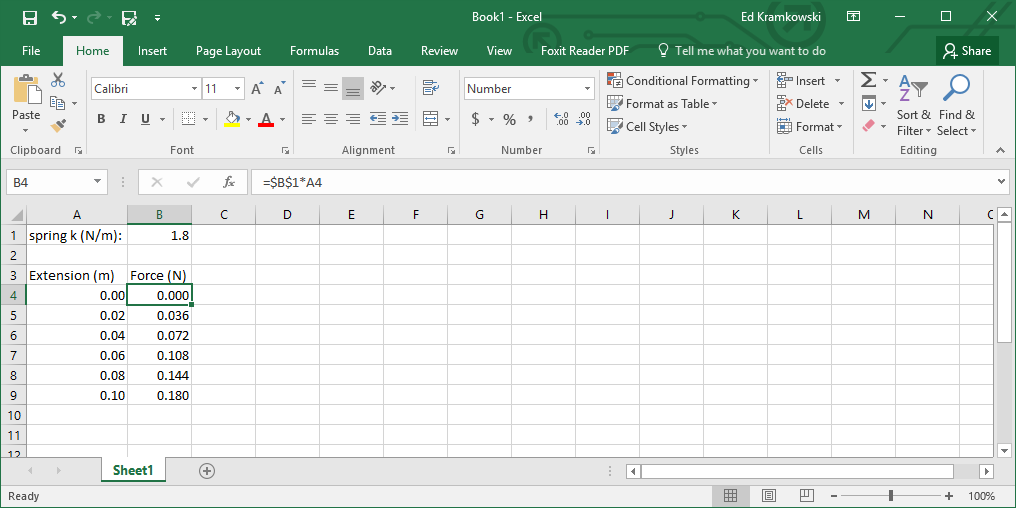
\includegraphics[scale=0.5]{excel1.png}
\centering
\caption{An example of using the \$ symbol to use a constant in a calculation. The force of a spring is calculated using $F=k * x$, where k is the spring constant and x is the extension of the springs length.}
\label{fig:exc1}
\end{figure}

Another example is shown in figure~\ref{fig:exc2} on page~\pageref{fig:exc2}.

\begin{figure}[ht]
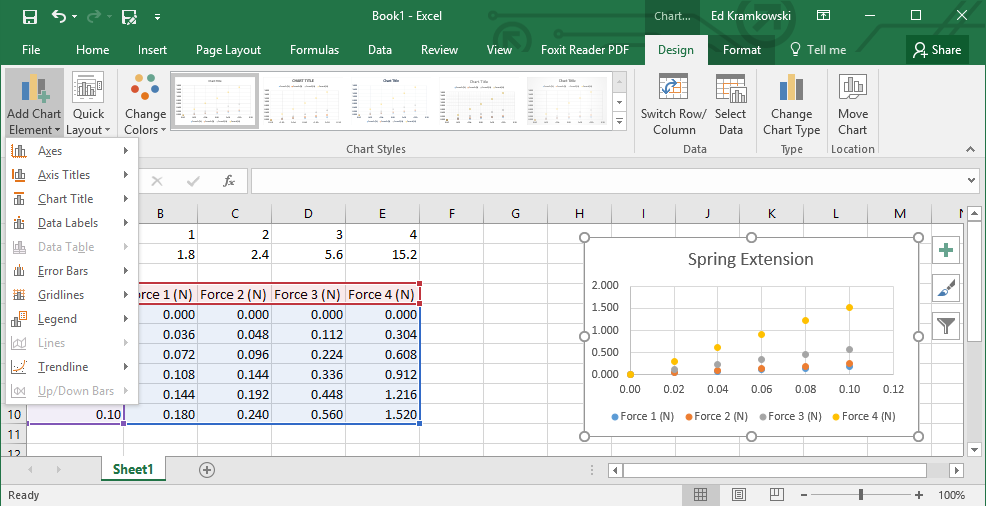
\includegraphics[scale=0.5]{excel4.png}
\centering
\caption{To add other elements to your chart (e.g. axis titles), choose ``Add Chart Elements'' from the ``Design'' menu.}
\label{fig:exc4}
\end{figure}

\section*{Generating Graphs:}
When creating a graph/plot, Excel will usually plot the first column on the independent/ horizontal axis and the second column on the dependent/vertical axis. 
You should always check that the correct data has appeared on the correct axis. 
If the data has been entered with the columns in reverse order, this can be fixed after the plot is created.
\par
To generate a graph/plot, use the mouse to highlight the data that you wish to graph (if the data is adjacent, just highlight the entire chunk; if the columns are not adjacent, highlight each column separately while holding the `Ctrl' key). 
Once the data is highlighted, click on the `Insert' tab and then the `Scatter' icon (on the `Charts' menu - other types of charts may be appropriate for different data types, but the Scatter plot is the most commonly used). 
From the sub-types of scatter plot available, choose the one that has data points but no lines. 
A graph will appear — but you are NOT finished yet!
\par
The design of the graph can be adjusted using the `Chart Layout' menu (see figure~\ref{fig:exc4}) - you will want to be able to label the individual axes with the quantity graphed and its units and you will want to be able to title the graph. 
When the graph has been titled (for the `vs.' format, it is always `Dependent' vs. `Independent') and the axes have been properly labeled, you can choose to keep or delete the Legend (not needed if only one data set is plotted, absolutely necessary for multiple data sets). 
The location of the chart can be changed by: left-clicking on the chart (the upper right corner works well), then right clicking and choosing `Move Chart' from the menu. 
It is often best to make the chart a `New Sheet' (so that it doesn't block your view of the data) - give it an appropriate title and click `Okay.' 
You chart will become its own sheet - and your data will disappear! 
But the data is not gone - to find it, use the tabs on the bottom of the Excel window (`Sheet 1' is usually the data; now might be a good time to rename it `Data': right click, select `Rename' and name it).
\par 
Before you finish, check that the correct data has been plotted on the correct axis and that the axis labels match the quantities plotted (see figures~\ref{fig:exc5} and \ref{fig:exc6}). 
If the original columns were in reverse order, this can be adjusted by left-clicking on a data point (to select the data), and then right-clicking and choosing `Select Data.' 
Click on the Legend Entry you wish to adjust, and then click `Edit.' 
Highlight the appropriate Series X and Series Y data and then click `Okay.'

\section*{Making Good Graphs}
One thing you should focus on in this class is developing good graph-construction habits.
Presenting data in a graph that is both accurate and easy to follow is an important skill to have in any scientific discipline. \\
When formatting your graphs:
\begin{itemize}
\itemsep-0.3em
\item Give your graph a descriptive title.
\item Make sure that all axes are labeled at a legible font size; do not forget to include units.
\item If you are graphing discrete data points (as will be the case most often), use only the basic scatter plot.
\item If your graph contains multiple independent data sets, be sure to include a legend.
\item Include a caption giving a short description of your graph. Make sure to note any important features.
\end{itemize}
\begin{figure}[ht]
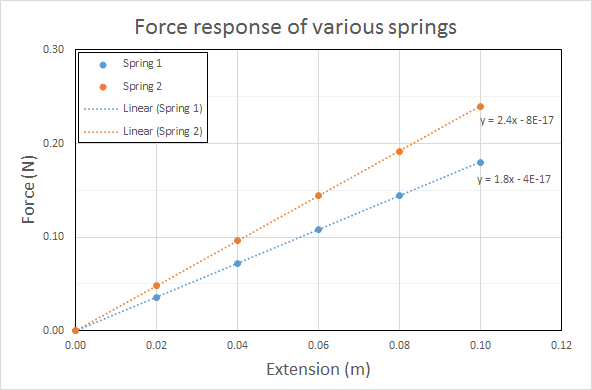
\includegraphics[scale=0.7]{excel3.png}
\centering
\caption{An example of properly graphed data. The data was plotted using a scatter plot. Trendlines (and their equations) were then added.}
\label{fig:exc3}
\end{figure}

\section*{Adding a Best Fit (``Trendline'') to a Graph:}
To add a line of fit (called a ``Trendline'' in Excel) to a graph:
\begin{itemize}
\itemsep-0.3em
\item Left-click on a data point to select the data series that you want to add a trendline for.
\item Right-click on the same data point and choose `Add Trendline.' 
\item The trendline formatting options should open on the right side of the program. Choose the appropriate Trend/Regression type, and tick the boxes for `Display Equation on chart' and `Display R-squared value on chart.' 
\item As a general rule, do not `Set Intercept' to a specific number (i.e., do not force the origin to be part of the trendline). 
\end{itemize}
Do you know what the R-squared value really means? 
If not, you should look it up! 
Look at the equation for the trendline and think about it. 
What does the slope mean? 
What does the y-intercept mean? What does this R-squared value mean?

\section*{Adding Error Bars to the Data Points on a Graph:}
Error bars represent the uncertainty of the measurement of the data. 
Do you have uncertainty? 
Do you have uncertainty in both quantities (horizontal and vertical)? 
Is the uncertainty the same for all data points, or does it change with the value of the quantity plotted? 
Wherever you have uncertainty, you must have error bars! 
Once you have determined the amount of uncertainty, you can add error bars by following these steps:
\begin{itemize}
\itemsep-0.3em
\item In the Chart Tool's `Design' tab, click `Add Chart Elements > Error Bars > More Error Bars Options...'. 
\item If you have multiple sets of data in the same chart, select the data series that you are adding error bars too.
\item The format window should open on the right. You can adjust the length of the error bars by selecting one of the options under `Error Amount'.
\item Apply the error bars according to the decisions that you have made about your uncertainty; a good choice is often `Standard Error', but you may sometimes wish to use errors that you calculated by selecting `Custom' and then selecting the appropriate cells with your errors. 
\item To remove either vertical or horizontal error bars, left-click on the bars, then right-click and choose `Delete'.
\end{itemize}

\section*{Other cool tools:}
As a spreadsheet program, Excel can do a lot of useful statistical analysis and mathematical manipulation. 
Some functions you will find useful include: Sum, Average, and Standard Deviation.
\par 
To \textbf{Sum} elements, click on the cell in which you wish the result to appear, then enter \texttt{=sum}. 
Immediately, Excel will list possible formula options that begin with \texttt{sum}. 
For a simple summation of elements, you would choose the SUM function, which you have already typed, but you should note the other options available. 
Open parentheses following your sum, so that you have now types \texttt{=sum(} and then highlight the cells to be summed. 
Close your parentheses and press `Enter.' 
(It would look like this \texttt{=sum(A1:A5)} for a sum of the cells in rows 1 through 5 of column A.)
\par 
To \textbf{Average} elements, click on the cell in which you wish the result to appear, and then enter \texttt{=average(}. Highlight the cells you wish to average and then close your parentheses and press `Enter.' 
Note that Excel will offer you a list of average functions - the most commonly used option is the AVERAGE function. (It would look like this \texttt{=average(A1:A5)} for the average of the cells in rows 1 through 5 of column A.)
\par 
To perform a \textbf{Standard Deviation} on a set of elements, click on the cell in which you wish the result to appear, and then enter \texttt{=stdev.s(}. 
Highlight the cells you wish to perform a standard deviation upon and then close your parentheses and press `Enter.' 
Note that Excel will offer you a list of standard deviation functions - the most commonly used option is the STDEV.S function. 
(It would look like this \texttt{=stdev.s(A1:A5)} for the standard deviation of the cells in rows 1 through 5 of column A.)
\par 
To perform any of these functions on disconnected sets of cells (e.g., cells in rows 1 through 13 and then 15 through 17), open your parentheses, highlight the first contiguous group, enter a comma, then highlight the next contiguous group, enter a comma, and so forth, continuing to the last group of numbers and ending with a closing parenthesis and the `Enter' key. 
(As an example, \texttt{=average(A1:A13,A15:A17)}.)
\par 
Excel has many other functions available, including trigonometric and logarithmic functions. 
Investigate what is available by clicking on the `Formulas' tab and looking through the `Function Library,' especially the `Math \& Trig' and `More Functions' menus.

\section*{Other Examples}

\begin{figure}[ht]
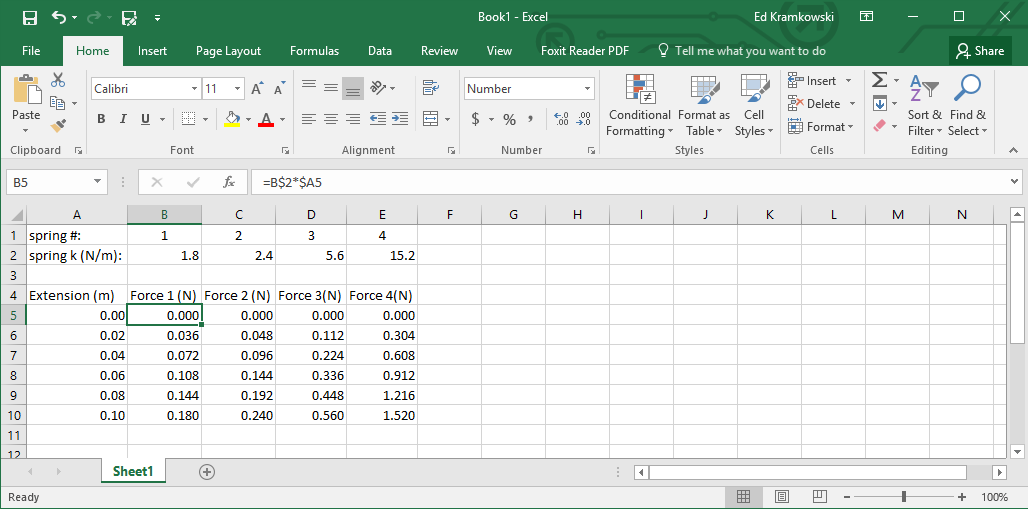
\includegraphics[width=0.8\textwidth]{excel2.png}
\centering
\caption{Another example of using the \$ symbol to use a constant in a calculation. By typing the formula \texttt{=B\$2*\$A5} into cell B5, you can allow the constant to change along a specified axis, while continuing to multiply by the numbers in the `Extension' column.}
\label{fig:exc2}
\end{figure}

\begin{figure}[ht]
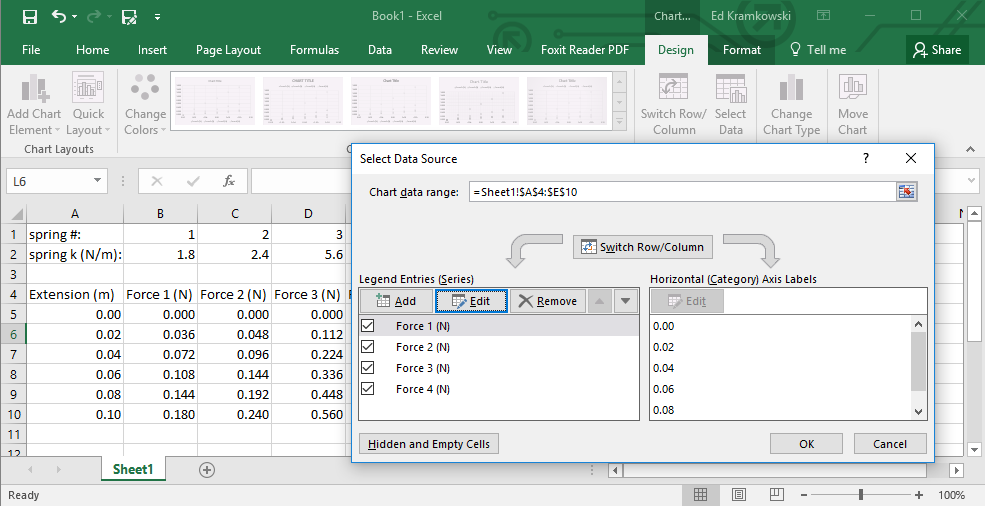
\includegraphics[width=0.8\textwidth]{excel5.png}
\centering
\caption{To edit or add sets of data to a graph, choose ``Select Data'' from the ``Design'' menu.}
\label{fig:exc5}
\end{figure}

\begin{figure}[ht]
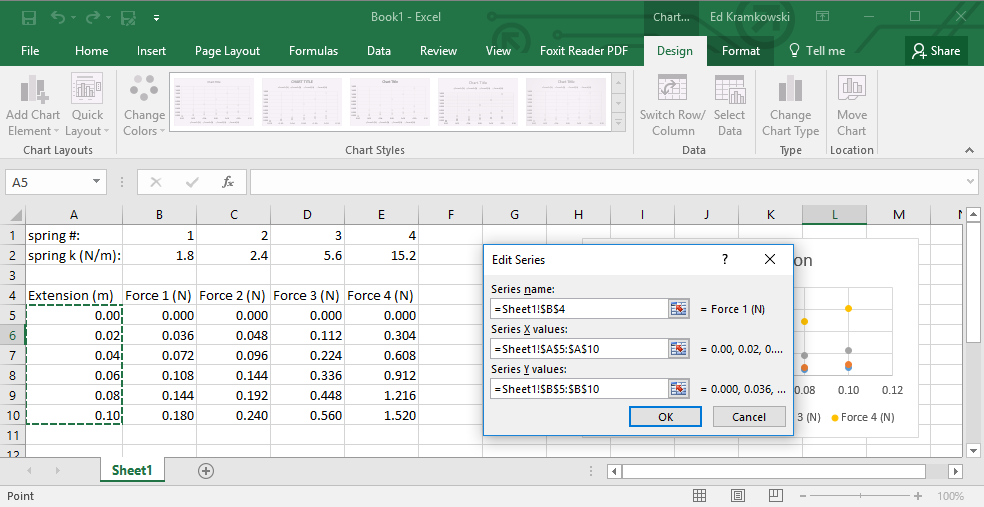
\includegraphics[width=0.8\textwidth]{excel6.png}
\centering
\caption{After selecting ``Edit'' in the ``Select Data Source'' menu, you can check if the values are being graphed on the proper axes, and edit the size of the data series if necessary.}
\label{fig:exc6}
\end{figure}	%\ref{chap:excel-analysis}
%\newpage{\blankpage}
\chapter{Creating Histograms in Excel}
\thispagestyle{fancy}
\fancyhead[RE,LO]{Technical Document \thechapter}
\label{chap:excel-hist}
%
There is more than one way to do this!
We will present two ways:
\begin{itemize}
\itemsep-0.2em
	\item Option \# 1: Using the Histogram Tool in the Data Analysis Package, and
	\item Option \# 2: Using the Frequency Function.
\end{itemize}
Choose whichever works best for you, given the settings available in your version of Excel.
%
\section{Using the Histogram Tool in the Data Analysis Package}
Excel has several `Add-Ins' that can be activated for the `Quick Access Toolbars.'
To see if the Data Analysis Add-In is activated on your version of Excel, click on the `Data' tab and look for this AddIn in the `Analysis' portion of the toolbar. 
(If it is not activated, you can try activating it by using the following steps: Position mouse over the `Data' tab and right-click; select `Customize Quick Access Toolbar...;' click on `Add-Ins;' Select Manage `Excel Add-Ins' and click `Go;' check the Analysis ToolPack and click `OK;' agree to activate the Add-In.
Now you should see the Data Analysis Add-In in the Analysis portion of the Data tab.)
\paragraph{Step 0: Make a plan!} 
Always have a plan in mind before you ask Excel to do anything! 
Looking at the full range of the data you wish to histogram, decide on a reasonable number of equal-sized bins and figure out what the boundaries of these bins should be. 
Type these boundaries into a column in Excel. 
(For example, if we histogram test grades, we might select bins ranging from 0 to 100 points, with 10 bins, each 10 points large. Here the bins are 0-10, 11-20, 21-30, 31-40, 41-50, ... 81-90, 91-100. These bin `boundaries' are 0, 10, 20, 30, 40, 50, ... , 90, and 100.)
\paragraph{Step 1: Activate the Histogram Analysis Tool.} 
Find the Data Analysis Add-In and click on it. 
Choose the `Histogram' analysis tool and click `OK.' Select the data you wish to create a histogram of and put this into the `Input Range' box. 
If you have decided what the boundaries of your bins will be, select the boundaries and put this into the `Bin Range' box. 
(If you don't enter anything into the Bin Range box, Excel will calculate these on its own — but, as we know, Excel does not always make good choices when left alone!) 
Click the `Output Range' bubble and enter a cell in your spreadsheet (this is where the results from the Histogram tool will be displayed). 
Then click `OK' and the analysis will be run.
\paragraph{Step 2: Understand the Histogram Output.} 
The Histogram analysis tool will output both Bin and Frequency data. 
An Example of such output is given here. 
The Frequency indicates the number of items from your data that fell between the previous and the current bin; i.e., a Frequency of 16 for Bin 10 says that the data you analyzed fell between the values of 5 and 10 a total of 16 times. 
The Bin `More' represents the number of times the data you analyzed has a value more than your maximum bin boundary; i.e., a Frequency of 0 for the More Bin indicates that none of the data you analyzed had a higher value than 25.
\paragraph{Step 3: Create the Histogram Plot.} 
Now you just need to make a bar graph of this data. 
Highlight the frequencies and click on the `Insert' tab, then click `Column' and select `2-D Column.' 
To adjust the horizontal axis labels, click on the plot, right click, and choose `Select Data,' then choose to edit the Horizontal Axis Labels. 
Title and label the plot appropriately. Tada!
%
\section{Using the Frequency Function}
Suppose you want to produce a histogram showing the distribution of student grades on a recent exam. 
The following guide outlines the procedure you would need to follow. 
\paragraph{Step 1:} Scan your data to get a sense for the overall range of values. 
For our example, the grades fall between 50 and 100, so this is the range that our bins must span. 
The next decision is how fine you want the increment of your bins to be — the finer the increment, the more bins, and thus the more bars in our histogram. 
For our sample data set, a bin increment of 10 seems appropriate. 
Create a column next to the raw exam score data that shows the bin ranges, and a column to the right of that which shows the maximum values of your bins. 
\paragraph{Step 2:} Now use the Excel function FREQUENCY to determine how many values fall within each of the bins that you have defined. 
The FREQUENCY function is an array function, returning values to a range of cells. 
Follow the following steps to enter the FREQUENCY function:
\begin{itemize}
\itemsep-0.3em
\item Highlight the range of cells which will hold the frequency counts (E2:E7). These will be all of the Frequency Count cells next to the max bin values.
\item Choose Insert $>$ Function..., pick the Statistical Function category and scroll down in the box on the right and choose FREQUENCY as the Function name.
\item Use the dialogue box to enter the function. With the Data\textunderscore array box selected, go to the spreadsheet page and highlight the data values (A2:A17). The dialogue box with ``roll up'' while you highlight these values and then ``roll down'' when you are done.
\item Repeat this process by selecting the Bins\textunderscore array box and then go out the spreadsheet and highlight the bin limits cells (D2:D7).
\item Click OK. The completed formula is seen in the formula bar and the correct count value is seen in the Bin Limit 50 count cell (E2).
\end{itemize}
\paragraph{Step 3:} Now copy the array function down to the other Frequency Count cells. 
This is a bit different than typical cell copying:
\begin{itemize}
\itemsep-0.3em
\item With the Frequency Count cells still highlighted (E2:E7), click on the FREQUENCY function into the formula bar (i.e., \texttt{=FREQUENCY(A2:A17,D2:D7)}).
\item Propagate the function by typing Control-Shift-Enter on a PC (type Command-Return on a Mac).
\end{itemize}
The frequency values should now fill the cells next to the bin increments. 
Note that your first bin increment, 50, holds all the grades at 50 and below. 
The next bin, 59, holds measurements from 50 - 59, and so on.
\paragraph{Step 4:} Create a bar chart plotting the frequency count (Column E) as a function of the student grade increments (Column C).		%\ref{chap:excel-hist}
\newpage{\blankpage}
\chapter{Measurement Error}
\thispagestyle{fancy}
\fancyhead[RE,LO]{Technical Document \thechapter}
\label{chap:error}
%
When getting quantitative information from a measurement, we are interested not just in the value
we obtain, but in how sure we are that the value we have measured is correct.
There are many factors that can produce a shift or an uncertainty in a measurement – we could have a meter stick with the end chipped off, our dials can only be read to a certain number of significant figures so the next digit is uncertain, or the setup conditions for our experiment can't be arranged precisely. 
In standard terminology these are referred to as ``errors'' – though this is a technical term that really means ``uncertainties.'' 
There is no implication that there are any mistakes made in doing the experiment!
Once we have a good estimate of how much uncertainty there is in our measurement, we estimate an error bar – a spread of values that says, ``We expect the odds are 2:1 that the actual value is inside this range.''
\par
Errors like our meter stick being chipped off and thus too short are called systematic errors. 
They always shift the result in one specific direction and need special care to reduce them.
Errors that arise from many small hard to control uncertainties (e.g. how well two fluids are mixed, how stable the temperature of the apparatus is, or whether the measurement is affected by building vibrations) are well studied mathematically and are referred to as random error, and these errors make the result bigger OR smaller in a RANDOM fashion. 
One way to get a handle on this random error is to repeat the experiment a number of times, preparing it as similarly as you can, and see how much variation there is. 
The statistical tools of mean (average) and standard deviation allow you to estimate both the average result and the error bar arising from random error.

\section*{Mean, Standard Deviation, \& Standard Error}
Given a number of measurements of the same event, the best estimate of the measurement is the mean of the values found,
\[ x_{best} = \bar{x} = \frac{1}{n} \sum_{i=1}^{n} x_{i} \]
where $n$ is the number of measurements.

A useful way of characterizing the reliability of the measurements is to calculate the standard deviation,
\[ \sigma = \sqrt{\frac{1}{n-1} \sum_{i=1}^{n}(x_{i}-\bar{x})^{2}} \]
The	significance of the standard deviation is that approximately 68\% of the measurements should lie within a range of $\sigma$ of the mean value.
With this definition, we can now write down the uncertainty of each individual measurement as $x_{i} \pm \sigma$.

The	mean of several measurements provides a better estimate of a quantity than a single measurement.
This stems from the fact that the uncertainty in the mean is smaller than the uncertainty of each individual measurement.
One can show that the uncertainty of the mean, also known as the standard error, is given by:
\[ \sigma_{m} = \frac{\sigma}{\sqrt{n}} \]
where $n$, again, is the number of measurements.

Then, the manner in which we will write the result of a set of measurements is that the best estimate and its uncertainty may be written
\[ x_{best} = \bar{x} \pm \sigma_{m} \]
The standard deviation of the mean slowly decreases with increasing number of  measurements; however, to improve the precision by a factor of 10, the number of measurements has to be increased by a factor of 100, which is hard work to say the least.
Thus, in practice, better precision is usually obtained by improving the experimental technique rather than just relying on an increased numbers of measurements.

\section*{Propagation of Error}
Often the measurement that we make is not the final answer we want. 
We may have to take a measured value as input in a calculation and do calculations with it. 
If there is uncertainty in the input numbers for our calculation, then there will be uncertainty in the output numbers as well – but they won't be the same uncertainty. 
The input and output numbers likely even have different units!
\par
To figure out how an input uncertainty translates into an output uncertainty, we simply have to ask: if the input value changed, how would that affect the output? 
We can answer that question by doing the calculation – changing the input value a little and calculating the changes in output. 
But we can also use calculus: the derivative of a function (an output calculated from some input) tells you how that output changes if the input changes a little! 
Mathematically these two options are written as follows:
\begin{equation}
\delta f = f(x + \delta x) - f(x)
\end{equation}
\begin{equation}
f(x + \delta x) = f(x) + \delta x \frac{df}{dx}
\end{equation}
Therefore we can write:
\begin{equation}
\delta f = \delta x \frac{df}{dx}
\end{equation}
We use the lower case delta ($\delta$) to represent a small change, since some of our inputs are changes already. 

\section*{General Form for Propagation of Error}
Let $\delta$x be the known uncertainty in x and $\delta$y be the known uncertainty in y. 
A function of x and y, such as f(x,y), will have two parts to its uncertainty — one contribution from x information and another contribution from y information. 
The contributions to the uncertainty of f are found using the relationships below:
\[ \delta f_{x} = \frac{df}{dx} \delta x \qquad \mathrm{and} \qquad \delta f_{y} = \frac{df}{dy} \delta y \]
The total uncertainty in f, $\delta$f, can be found by using the relationship:
\begin{equation}
\delta f = \sqrt{(\delta f_{x})^{2}+(\delta f_{y})^{2}}
\end{equation}

\subsection*{Example 1: Average Velocity}
If you know the uncertainty in $\Delta$x, $\delta$($\Delta$x), and the uncertainty in $\Delta$t, $\delta$($\Delta$t), then you can use the formula for average velocity, $\langle v \rangle = \frac{\Delta x}{\Delta t}$, to find the uncertainty in the average velocity, $ \delta (\langle v \rangle)$.
\[ \delta \langle v \rangle_{\Delta x} = \frac{d \langle v \rangle}{d(\Delta x)} \delta (\Delta x)
   \quad \rightarrow \quad \mathrm{compute \ derivative} \quad \rightarrow \quad
   \delta \langle v \rangle_{\Delta x} = \frac{1}{\Delta t} \delta (\Delta x)\]
%
\[ \delta \langle v \rangle_{\Delta t} = \frac{d \langle v \rangle}{d(\Delta t)} \delta (\Delta t)
   \quad \rightarrow \quad \mathrm{compute \ derivative} \quad \rightarrow \quad
   \delta \langle v \rangle_{\Delta t} = \frac{-\Delta x}{\Delta t^{2}} \delta (\Delta t)\]
%
\[ \delta \langle v \rangle = \sqrt{(\delta \langle v \rangle_{\Delta x})^{2} 
   + (\delta \langle v \rangle_{\Delta t})^{2}} = \sqrt{\left(\frac{1}{\Delta t} \delta (\Delta x)\right)^{2} + \left(\frac{-\Delta x}{\Delta t^{2}} \delta (\Delta t)\right)^{2}} \]

\paragraph{For example,} let say that want calculate the average velocity of a air-track cart. Your track is 2 m long, and the error you estimate for your meter stick is 5 mm. You used a photogate system to measure the time it took for the cart to traverse the track; you measured a value of 4.0  with an error of 0.3 s. Thus, your average velocity would be 0.5 m/s, and your uncertainty would be:

\[ \delta \langle v \rangle = \sqrt{ \left( \frac{1}{4.0 \, s} (0.005 \, m) \right)^{2} + \left( \frac{-2.0 \, m}{(4.0 \, s)^{2}} (0.3 \, s) \right)^{2}} = 0.038 \, m/s \]
Thus, you would report the average velocity of your cart as $v = 0.5 \pm 0.038 \, m/s$

\subsection*{Example 2: A Sinusoidal Function}
Given a sinusoidal function $a = \sin(\omega t) + 2$ and uncertainties in $\omega$, $\delta \omega$, and in t, $\delta$t, the uncertainty in a, $\delta$a can be calculated as follows:
 \[ \delta a_{\omega} = \frac{da}{d \omega} \delta \omega
   \quad \rightarrow \quad \mathrm{compute \ derivative} \quad \rightarrow \quad
   \delta a_{\omega} = t \cos(\omega t) \delta \omega \]
%
\[ \delta a_{t} = \frac{da}{dt} \delta t
   \quad \rightarrow \quad \mathrm{compute \ derivative} \quad \rightarrow \quad
   \delta a_{t} = \omega \cos(\omega t) \delta t \]
%
\[ \delta a = \sqrt{(\delta a_{\omega})^{2} + (\delta a_{t})^{2}} 
   = \sqrt{\left( t \cos(\omega t) \delta \omega \right)^{2} + \left( \omega \cos(\omega t) \delta t \right)^{2}} \]
   
\section*{Why Propagate Error}
We often hear students express the following frustrations: "What's the big deal with all of
this error analysis, anyway? Is it just busy work? Is there a more significant, scientific purpose?
Why are there so many ways to determine error??!?"
\par
\textbf{Error analysis is key to science and medicine.}
The key question in medical research and medical practice is, whether a treatment works! 
Does a new drug make a patient feel better or remove their disease better than another treatment? 
To answer this question requires comparing observations before and after, or comparing treated patients with so called ``controls'' in clinical trials. 
But how can we tell whether something is the same or different? 
This is where error analysis comes in as a crucial stepping stone!
\par
We randomly chose an article on a medical topic (cancer therapy) from a recent issue of the prestigious journal Nature. 
In all of the four figures included in the article, we saw that the authors, in trying to show that their therapy works, compared mice that were treated with their therapy to ``controls,'' i.e.\ untreated mice as shown in the sample image on the right. 
To highlight a statistically significant difference it is customary to put a ``star'' in the figure. 
In this figure you see two stars showing that the two images on the left are different, and the two images on the right are different. 
But how would you determine that the two x-ray images are different? 
Use error analysis and error propagation! 
In this example the input data are x-ray images, which have uncertainty from mouse to mouse and from x-ray exposure to x-ray exposure. 
The output, which is what the authors want to compare, are ``tumor to background ratios.''
\par 
\textbf{Our take home message:} Error analysis is the hidden backbone of scientific research. 
It may only show up as small stars in an otherwise glossy image, but without that star the authors could not draw any conclusion from these images other than ``each mouse has a somewhat different number of tumors.'' 
Overall we counted 38 ``stars'' in the article that analyzed the effectiveness of one particular therapy! 
\textbf{We want you to become Stars of Error analysis!}
\par 
\textbf{There ARE a lot of ways to do error analysis.} 
Part of what you are learning to do, as budding scientists and doctors, is to find a way to choose the method of error analysis that best matches the experimental design/protocol. 
There is no single `formula' for error analysis, just as there is no single `formula' for doing science! 
Here are some error analysis methods that you will encounter in this class:
\begin{itemize}
\item determine uncertainties in individual measurements and propagate error to find the output error (as described in this document); or,
\item calculate the output for each input from the multiple trials and use the standard deviation of the output to establish the uncertainty of the output directly.
\item (There ARE other methods, but these are the most commonly used....)
\end{itemize}		%\ref{chap:error}
\newpage{\blankpage}
\chapter{How to use ImageJ}
\thispagestyle{fancy}
\fancyhead[RE,LO]{Technical Document \thechapter}
\label{chap:imagej}

\section{Basic ImageJ tasks}

\subsection*{Opening an image}
To open an image, either:
\begin{itemize}
\itemsep-0.3em
\item Click `File $>$ Open', and then navigate to the image you wish to analyze.
\item Drag and drop the image you wish to analyze onto the main ImageJ window.
\end{itemize}
To open a video file:
\begin{itemize}
\itemsep-0.3em
\item Click `File $>$ Import $>$ AVI...'. Select the video you wish to import then click `Okay'.
\item In the `AVI Reader' window that opens, select the `Convert to Grayscale' option, and click `Okay'.
\end{itemize}
After importing a video file, you may need to edit it in order to allow our tracking tool to properly follow different features.
\begin{itemize}
\itemsep-0.3em
\item Once you have selected an appropriate area, highlight this area with the *Rectangle* selection tool, click on `Image $>$ Crop'. 
This will delete the rest of the video, and leave only the relevant section. 
If you want, you can use the zoom button (`Ctrl + ``+''') to make this selection a bit larger on your screen.
\item Now that we have an appropriate video, we need to process it to the point of being black features on a white background, with limited noise. 
The first step is set the threshold for the video, which basically takes all of the shades of gray in the video and turns it into black or white. 
To do this:
\begin{itemize}
\item Click on `Image $>$ Adjust $>$ Threshold'. 
\item In the menu that pops up, play with the sliders until the featrures you are investigating are displayed in black, but there is no black elsewhere in the video. 
It should look similar to the screenshot. 
\item Once you have achieved this, click on the apply button. 
Apply the threshold to all of the frames of the video, but you don't have to calculate it each time, the first is enough. This should produce images similar to the one in the screenshot, with black spots on a white background.
\end{itemize}
\item You may notice that there are some little spots of noise around your images. 
To fix this:
\begin{itemize}
\item Go to `Image $>$ Adjust $>$ Contrast'.
\item Set the contrast tab all the way to the right.
\item This should further separate the difference between black and white, leaving just the black spots of the beads
\end{itemize}
\end{itemize}
\subsection*{Determining distance-to-pixel ratio in ImageJ}
Once you have imported a file into ImageJ, you will need to determine the distance-to-pixel ratio for your video (this should be done separately for each image/video analyzed). 
\begin{itemize}
\itemsep-0.3em
\item You will need to use the `line' tool (*Straight* tool, 5th from left end of icons in toolbar) in ImageJ.
\item Click on the `line tool' icon of the ImageJ menu toolbar (it looks like a sloped line or a slanted fraction bar (/), and the bottom right corner has a downward-pointing black triangle). 
\item Using this tool, click on one end of a `known length’ object hold down the mouse button, and drag the line across the `known length’ object to the other side. 
\item Click `Analyze $>$ Set Scale...'. Edit `Known Distance' and `Unit of length'. Now that the scale is set, the rest of the measurements that you take will be reported in the entered units.
\end{itemize}

\section{How to use ImageJ automatic tracking}
The main difference between manual and automatic tracking is the preliminary image processing that is required. 
It takes longer to prepare each video for analysis, but automatic tracking makes it much easier to quickly track many particles. 
Essentially, our goal will be to process our image sequence to the point where our particles appear as black spots on a white background.

\subsection*{Gathering Data with the Automatic Tracking Plugin}
Once you have processed your video, you can open the Automatic Tracking plugin. 
The Automatic Tracking plugin allows you to collect horizontal (X) and vertical (Y) position coordinates for objects at different times within the video automatically by only describing the sizes of the objects you want to look at. 
To activate the Automatic Tracking plugin:
\begin{itemize}
\itemsep-0.3em
\item Click on `Plugins $>$ 2131\_Plugins $>$ MultiTracker'. A new window will appear. 
\item Adjust the min and max size if necessary to exclude any noise in your video. 
Because of the way we processed the image, the only objects in the video should be the beads we are looking at, so these parameters should work.
\item If you would like a clearer idea of which bead is which, and where they move over time, you can select the Show Label/Path options.
\end{itemize}

\subsection*{Exporting the Automatic Tracking Data to Excel}
When the data collection is finished, go to your data window and examine how many different particles were tracked for the video. 
The columns of the resulting data table will just be the X and Y positions for each of the particles that the computer identifies.
\begin{itemize}
\itemsep-0.3em
\item Make sure that you only use data for real beads displaying real random motion. 
You can check this by identifying the object at each coordinate position in the result table. 
If the computer recognized noise as a bead, make sure you exclude this from your analysis. 
\item If a bead enters or leaves the screen, make sure you exclude this point as well. 
\item If a bead is clearly stuck to the slide and not moving at all, you may want to consider excluding that data point. 
\item Once you are sure that you have identified the beads in your results table, you can save your results into an excel file (Option 2 is best for this, as there will be MANY columns).
\begin{itemize}
\item Option 1: `Edit' $\rightarrow$ `Select All' $\rightarrow$ `Ctrl' + `C' to Copy $\rightarrow$ Paste into an Excel file (you must add the column titles yourself), or
\item Option 2: `File' $\rightarrow$ `Save As...' $\rightarrow$ Name the file what you will and click `Save'. (It will save in Excel format with column titles.)
\end{itemize}
\end{itemize}	%\ref{chap:imagej}
\newpage{\blankpage}
%\chapter{Introduction to Video Capture}
\thispagestyle{fancy}
\fancyhead[RE,LO]{Technical Document \thechapter}
\label{chap:vid-cap}

\section*{Finding the software on the lab computer}
The software should be clearly available on the desktop. 
If it is not, go to the start menu and type `virtual' into the Search Programs and Files box. 
The software you want is called `VirtualDub' and has an icon that looks like a gray gear-and-screw. 
Open this.

\section*{Capturing video with the webcam}
\begin{itemize}
\item The fist window that opens is for editing videos. Select `File $>$ Capture AVI' to open the video capture window.
\item If both a webcam and a microscope are connected to your computer, you may need to select the device. 
Select `Device,' and `Microsoft LifeCam Studio (TM) (DirectShow)' for the webcam or the `Toupcam (DirectShow)' option for the microscope.
\item If you do not see the output from the camera showing in the window, make sure that `Video $>$ Preview' is checked.
\item There are a number of settings that you can investigate to change aspects of the video you wish to capture.
Your lab station will have a guide with more information about recommended settings to use, what settings you may need to adjust, and what settings should not be changed.
\item Be aware that ImageJ can process only about 400 frames (due to the limited working memory of the computer, more frames possible with the virtual stack option), so you will need to adjust the play rate and total time of your video to take the minimum length to capture your event and not much else. This can be done very easily in the VirtualDub editing window.
\item Check the save location, file name, and auto-increment settings so that you don't lose any data and avoid writing over anyone else's data.
\item When you are ready to capture video of motion/your subject, select `Capture video' or press F6. Once your experiment is complete, click `Stop Capture' or press `Esc' to stop recording.
\item Keep in mind, you may need to collect several trial videos before you manage to get good video for analysis in ImageJ.
\end{itemize}

\section*{Editing captured videos}
As mentioned before, it is often a good idea to edit your videos after capturing them.
Even short captures can result in large file sizes, so in order to expedite the analysis of your videos and to reduce the amount of space you need to store your data you shoulds edit your videos after you are done capturing your data.
Fortunately, VirtualDub's video editing software is a very simple to use.
\begin{itemize}
\item Go to `File $>$ Open video file...' and select the file you want to edit.
\item Use the left and right arrow keys to scroll through the video frame-by-frame; locate the are that you plan on analyzing.
\item Navigate to a frame a few before the ones that contain your data. Click the `End' key to select all of the opening video that you wish to delete, then click the `Delete' key to remove it.
\item Don't worry if you make a mistake, nothing is saved until you click `File $>$ Save as AVI...'. If you accidentally erase the wrong frames, select `File $>$ Close video file' and then start again from the beginning.
\item If there is any video you wish to remove from the end of your file, move to a few frames after your data and click the `Home' key, then move to the end of the video and click the `End' key, then click `Delete'.
\item Once you have deleted the majority of the unnecessary frames, select `File $>$ Save as AVI...' to save your edited video. Note that you cannot use the same filename as the video you currently have open.
\end{itemize}

\section*{Video construction \& planning}
Creating a good video for analysis in ImageJ is tougher than you might think. 
You will need to consider elements of video construction and planning. 
You need to be a ‘Good Cinematographer.’ 
Here are some questions to consider:
\begin{itemize}
\item What is the best angle? How should the camera be aligned to view the motion of the object
in which you are interested?
\item What is the best time between frames? How many frames-per-second should you be collecting, given the time for the phenomena to occur and the memory limitations of ImageJ (about 400 frames)?
\item Is there a known length visible in the video?
\item Are all objects of interest clearly visible in the video?
\item Is the entire portion of motion in which we are interested visible in the video?
\item Is the camera (perspective) stationary?
\end{itemize}

		%\ref{chap:vid-cap}
%\newpage{\blankpage}
\chapter{Microscope Basics}
\thispagestyle{fancy}
\fancyhead[RE,LO]{Technical Document \thechapter}
\label{chap:scope-basic}

\section*{Microscope Parts}
Below is a list of the different parts of the microscope and their function.
If you are having trouble identifying a particular part, or are unsure of how to operate something, ask your TA for assistance.

\begin{figure}[ht]
	\centering
	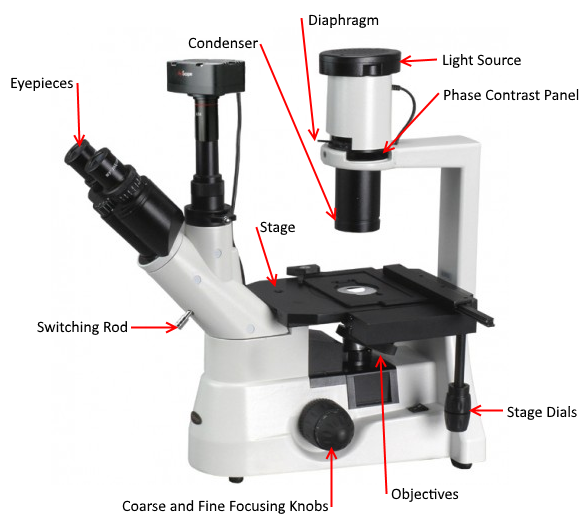
\includegraphics[scale=0.7]{microscope.png}
	\caption{Diagram of the microscope parts.}
	\label{fig:microscope}
\end{figure}

\begin{itemize}
\itemsep-0.3em
\item Eyepieces
\begin{itemize}
	\itemsep-0.3em
	\item Adjustable to fit both eyes. If eyelashes obstruct view, move closer to the eyepieces.
%	\item Sometimes easier if one eye is closed
\end{itemize}
\item Light Source, Condenser, Phase Contrast Panel
\begin{itemize}
	\itemsep-0.3em
	\item Condenser concentrates light from illumination source.
	\item Phase rings in front of the light source allow the microscope to translate phase shifts in light that goes through a transparent sample into brightness changes in the observed images. This allows for very useful imaging of transparent samples that would be difficult with standard bright field imaging.
	\item The light intensity can be controlled by adjusting the orange wheel on the bottom left of the machine.
\end{itemize}
\item Diaphragm
\begin{itemize}
	\itemsep-0.3em
	\item Lever controls an iris, allowing the user to control the amount of light hitting the sample. Very often, higher detail can be observed by allowing less light through the iris.
\end{itemize}
\item Stage
\begin{itemize}
	\itemsep-0.3em
	\item Place the sample on the microscope stage carefully. The stage can be moved relative to the objectives using the dials below the stage to the right. Align the sample directly over the objective, so the light is shining directly on the sample.
\end{itemize}
\item Objectives
\begin{itemize}
	\itemsep-0.3em
	\item Objectives collect the light from the samples and focus it to form an image in the eyepiece or CCD camera. Rotating turret holds four different objective lenses: 4X, 10X, 20X, and 40X. Always start with a low magnification objective: find, center, then focus on the sample before moving on to a higher magnification.
%	\item Always lower objectives using the coarse adjustment knob before rotating the turret.
\end{itemize}
\item Coarse and Fine Focusing Knobs
\begin{itemize}
	\item Bring sample into view using the coarse adjustment knob (inner knob). Once sample is in view, use the fine adjustment knob (outer knob) to achieve the sharpest possible image. Be careful when using the coarse adjustment knob, hitting the slide with the objective can scratch the objective or crack the slide.
\end{itemize}
\item CCD Camera
\begin{itemize}
	\itemsep-0.3em
	\item Adjust the switching rod to go from eyepiece-only to dual-view mode. Camera can be rotated using the adjustable pin below the lens
\end{itemize}
\end{itemize}

\newpage

\section*{Microscope Software}
The capture software for the microscope is called ``Amscope'', it should be located on the desktop.
The software has a viewing area in the center and adjustment settings on the left.
To begin, click `MU503' under `Camera List' to see the view from the camera in the viewing area.
Then adjust the following settings:
\begin{itemize}
\itemsep-0.3em
\item Set the `Live' and `Snap' resolutions. While capturing video it's best to use `1280 x 960'.
\item Uncheck `Auto Exposure'. Adjust the `Exposure Time' to approximately 33 ms, this means you will be capturing video at 30 fps. Turn the Gain down to 1.0, increase this if you cannot get a bright enough image.
\item In `Color Adjustment', reduce Saturation to 0 and Contrast to 100. Adjust the brightness as necessary.
\end{itemize}
\paragraph*{To capture a video:}
See figure~\ref{fig:am-cap} while following along with the steps below:
\begin{itemize}
\itemsep-0.3em
\item Click the `Record' button on the left, this will open a window called `Video file'.
\item Type the name of the video file that you want to capture; select your group's data folder as the save location. Click Next
\item Select the `avi' format, click Next.
\item Under `Encoder' setect `None Compressor', leave the encode parameter quality set at 100. Click Next.
\item Check the box next to `Time Limit', then input the number of seconds that you want to capture video. Clicking `Finish' (or pressing Enter) will begin the video capture.
\end{itemize}
The microscope can be very sensitive to table vibrations, especially when you are imaging at high magnifications. 
After setting all the video capture parameters, wait a bit before starting the capture for the vibrations to die down.
While the camera is capturing, do your best to not disturb the table.

\paragraph*{To capture a `low fps' video:}
Occasionally we may need to capture video at a low frame rate over a long period of time.
To do this, we will set the software to capture an image every few seconds (see figure~\ref{fig:low-fps}).
Then, we will use ImageJ to stitch the images together into a .avi video.
\begin{enumerate}
\itemsep-0.3em
\item Navigate to `Capture $>$ Start Time-lapse (Auto Capture)...'
\item In the window that opens, adjust the following settings:
	\begin{itemize}
	\itemsep-0.3em
	\item Directory
		\begin{itemize}
		\itemsep0em
		\item Base: Choose an empty folder within your group's data folder.
		\item Sub: Leave as none.
		\end{itemize}
	\item File
		\begin{itemize}
		\itemsep0em
		\item Name Format: Set to `nnnn (sequence)'.
		\item File Prefix: Input the names that you want given to the images.
		\item File Type: Set to png.
		\end{itemize}
	\item Capture Mode
		\begin{itemize}
		\itemsep0em
		\item Select `Time Slot' and input the number of seconds between each frame.
		\end{itemize}
	\item Check `Total Images', then input the number of frames that you want captured.
	\end{itemize}
\item Clicking OK or pressing Enter will begin the time-lapse. As before, wait for the vibrations to die down before beginning the capture, and avoid touching the table.
\item After the time-lapse is complete, open ImageJ and navigate to `File $>$ Import $>$ Image Sequence...'.
\item Navigate to the folder where your time-lapse images are saved, choose any of the images and click Open.
\item In the Sequence Options window, make sure `Sort names numerically' is checked, then click OK.
\item After processing the images, a new window will open. Navigate to `File $>$ Save As $>$ AVI...'. Set Compression to `Uncompressed', set Frame Rate to 25, click OK. Enter the file name, then press Save.
\item After creating the avi file, delete the time-lapse images to avoid using unnecessary space.
\end{enumerate}

\begin{figure}[hb!]
	\centering
	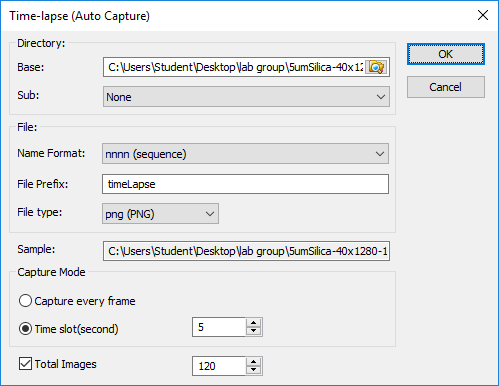
\includegraphics[width=0.55\textwidth]{amscope06}
	\caption{Example Amscope `low fps' video capturing settings.}
	\label{fig:low-fps}
\end{figure}

\begin{figure}[ht]
	\centering
	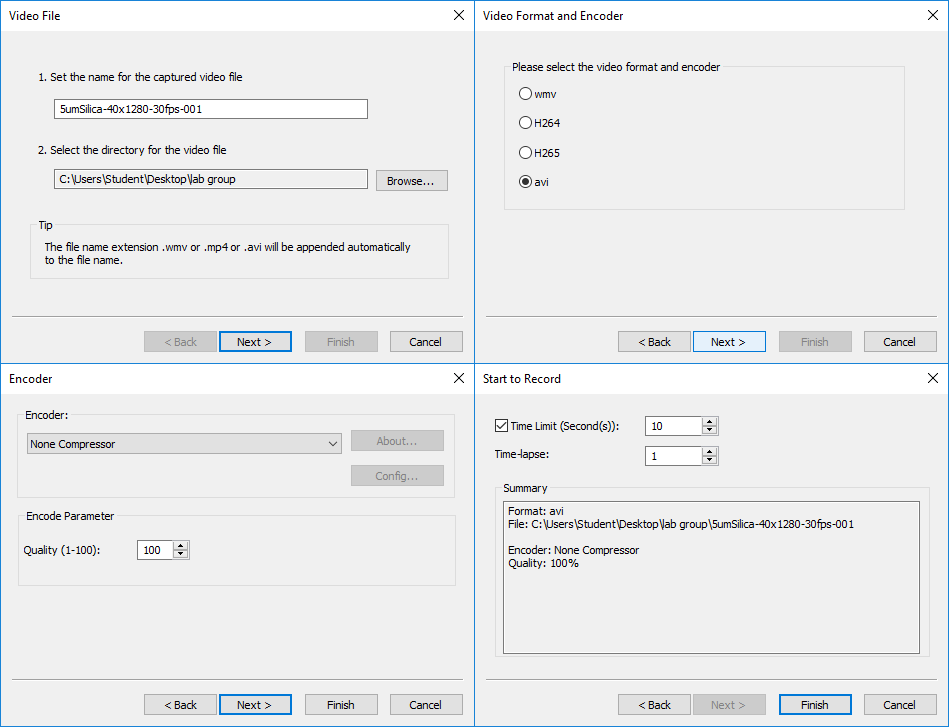
\includegraphics[width=\textwidth]{amscope08}
	\caption{Amscope video capturing settings.}
	\label{fig:am-cap}
\end{figure}

%\section*{Eyepieces:}
%\begin{itemize}
%	\setlength\itemsep{1pt}
%	\item Adjustable to fit both eyes
%	\item Sometimes easier if one eye is closed
%	\item If eyelashes obstruct view, move closer to the eyepieces
%\end{itemize}
%
%\section*{Light Source, Condenser, Phase Contrast Panel:}
%\begin{itemize}
%	\setlength\itemsep{1pt}
%	\item Condenser concentrates light from illumination source
%	\item Phase rings in front of the light source allow the microscope to translate phase shifts in light that goes through a transparent sample into brightness changes in the observed images. This allows for very useful imaging of transparent samples that would be difficult with standard bright field imaging.
%	\item The light intensity can be controlled by adjusting the orange wheel on the bottom left of the machine.
%\end{itemize}
%
%\section*{Diaphragm:}
%\begin{itemize}
%	\setlength\itemsep{1pt}
%	\item Lever controls an iris, allowing the user to control the amount of light hitting the sample
%	\item Very often, higher detail can be observed by allowing less light through the iris
%\end{itemize}
%
%\section*{Stage:}
%\begin{itemize}
%	\setlength\itemsep{1pt}
%	\item Place the sample slide on the microscope stage carefully
%	\item The stage can be moved relative to the objectives using the dials below the stage to the right
%	\item Align the sample directly over the objective, so the light is shining directly on the sample
%\end{itemize}
%
%\section*{Objectives:}
%\begin{itemize}
%	\setlength\itemsep{1pt}
%	\item Objectives collect the light from the samples and focus it to form an image in the eyepiece or CCD camera.
%	\item Rotating turret holds four different objective lenses: 4X, 10X, 20X, and 40X
%	\item Always start with a low magnification objective: find, center and focus on the sample before moving on to a higher magnification.
%	\item Always lower objectives using the coarse adjustment knob before rotating the turret
%\end{itemize}
%
%\section*{Coarse and Fine Focusing Knobs:}
%\begin{itemize}
%	\setlength\itemsep{1pt}
%	\item Bring sample into view using the coarse adjustment knob (inner knob)
%	\item Once sample is in view, use the fine adjustment knob (outer knob) to achieve the sharpest possible image.
%	\item Be careful when using the coarse adjustment knob, hitting the slide with the objective can scratch the objective or crack the slide.
%\end{itemize}
%
%\section*{CCD Camera:}
%\begin{itemize}
%	\setlength\itemsep{1pt}	
%	\item Camera can be rotated using the adjustable pin below the lens
%\end{itemize}		%\ref{chap:scope-basic}
\newpage{\blankpage}
\chapter{Log-Log Plots}
\thispagestyle{fancy}
\fancyhead[RE,LO]{Technical Document \thechapter}
\label{chap:log-plots}

In understanding how one variable depends on another, we introduced the idea of \emph{functional dependence}.
This helps us understand not just that one variable depends on another, but how it depends on the other.
This is especially important in complex situations such as biology where many variables can be involved and "which one dominates" matters.

\section{Powers \& Exponents}

\subsection*{Powers}
Some of the most useful and convenient functional dependencies that we will encounter are \textbf{power laws}.
This means that the variable we choose to be `dependent' depends on the variable we choose to be `independent' by some power of that variable.
Thus
\[ y = f(x) = x^{N} = x \text{ multiplied by itself } N \text{ times} \]
says that ``\emph{y goes like x raised to the Nth power}''.
Note that a power law is not referred to as an ``exponential dependence'' even though the variable ``has an exponent''.
That terminology is reserved for the case when the variable is in the exponent.

\subsection*{Exponentials}
We know that a quadratic function rises faster than a linear one (eventually) and a cubic rises faster than a quadratic.
But there is an extremely useful function that eventually rises faster than any power.
This is the exponential function.
In this case, the variable is not raised to a power - the variable itself is in the power that some constant is raised to.
So as the variable gets bigger and bigger, the power the constant is raised to gets bigger and bigger.
\par
We write
\[ y = e^{x} \text{.} \]
Now e could be any constant, but we typically take it as a special transcendental number (that means it's decimal representation never stops and never repeats): $e = 2.712...$

\subsection*{Logarithms}
The exponential function does the interesting thing of converting sums into products.
If $R = e^{a}$ and $S = e^{b}$ then $R \cdot S = e^{a+b}$.
So if $f(x) = e^{x}$ then we have
\[ f(x_{1})f(x_{2}) = f(x_{1} + x_{2}). \]
Since multiplying is harder than adding, it's sometimes useful to go backwards from the exponential function. 
Taking the exponential of $x$ and setting $y = e^{x}$, if we are given $x$ we can use our calculator (or series) to find $y$.
But what if we are given $y$ and want to find $x$?
The answer to that is called the \emph{natural logarithm} of $y$.
So that would give us the equation:
\[ x = ln(y) \]
Plugging this equation back into our original equation gives:
\[ y = e^{ln(y)} \]
This shows that the natural log ($ln$) is the \emph{inverse function} of the exponential.
If we first take the natural log and then exponentiate it, we get back what we started with.
It works the other way too:
\[ x = ln(e^{x}) \]
If we exponentiate first and then take the natural log, we get back what we started with.
So the natural log function ($ln$) undoes the exponential function and vice versa.
We will see in the following sections that logarithms and exponentials are very useful in analyzing data and seeing whether something behaves like a power law. 

\section{Log-Log Plots}
Power law equations are often used in science to approximate more complicated functions.
%When we have a complicated function it is sometimes useful to approximate it by a simple power law.
However, when these types of equations are plotted on a standard linear graph it can be difficult to recognize the differences between two functions with similar (but not equal) powers.
What we need to do is perform an easily-invertible operation on all our data that also emphasizes changes in power laws. 
One way to see how to do this is to use a \emph{log-log plot}.
Instead of just plotting the variables themselves, we plot the logarithm of the variables.
Let's see how this works.
\par
Suppose we have a power law function $y = ax^{N}$.
If we plot this, we get curves like those in the left side of figure~\ref{fig:lin-log}.
The higher the power we have, the faster it rises (and the odd powers are negative for negative values of x.)
But if we take the logarithm of both sides of that equation, $y = ax^{N}$,we get
\[ log(y)=N \cdot log(x) + log(a) \] 
If we now take as new variables $Y = log(y)$, $X = log(x)$, and $b = log(a)$ then our new equation is just
\[ Y = N \cdot X + b \]
This is the graph of a straight line and the slope is proportional to the power.
If we plot this we get the graph at the right in figure~\ref{fig:lin-log}.

\begin{figure}[ht]
	\centering
	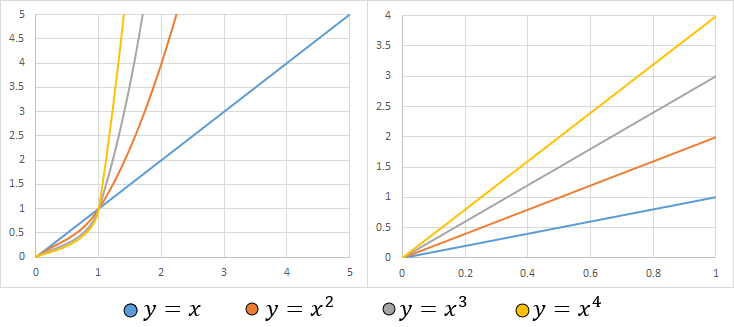
\includegraphics[width=0.8\linewidth]{linVSlog.png}
	\caption{Comparison of linear vs. log-log graphs.}
	\label{fig:lin-log}
\end{figure}

\newpage

All the power laws are straight lines with increasing slope as the powers go up.
So if we are interested in determining if some complicated function can be approximated by a power law, we can easily see if this is the case by plotting the logarithms of the variables. 
If we get a straight line, a power law works. 
(We have only plotted positive values of x and y in the log-log plot since the log of a negative number is not a real number.
Note that this works for negative powers too.) 

%\section{Log-Log Plots in Science}
%Log-Log plots have many uses in science.
%They are especially helpful for differentiating between different forms of \emph{functional dependency}.
%What is functional dependency? 
%Functional dependency tells us how one quantity varies when another is adjusted. 
%Example: for purely random motion, the diffusion of an object in 2-D space has a functional dependence like $\langle r^{2} \rangle = 4 D \Delta t$. 
%As you saw in lab, the viscosity and temperature of the fluid medium surrounding the object and the size of the object can affect the value of the diffusion constant, D, and thus the linear slope of the $\langle r^{2} \rangle$ vs.\ $\Delta t$ plot (where the slope is related to D). 
%A $log(\langle r^{2} \rangle)$ vs.\ $log(\Delta t)$ plot of this functional dependency would be a line with a slope of 1 — regardless of the value of the diffusion constant, D! 
%If we are not learning the diffusion constant D from this log-log plot, what does the slope of 1 tell us?
%\par 
%It turns out that the slope of $log(\langle r^{2} \rangle)$ vs.\ $log(\Delta t)$ tells us about what type of motion we are observing! 
%Most motion will not be linear in an $\langle r^{2} \rangle$ vs.\ $\Delta t$ plot. 
%There are other functional dependencies that can exist governing the relationship between $\langle r^{2} \rangle$ and $\Delta t$. 
%For directed motion at constant velocity, $\langle r^{2} \rangle$ changes as $(\Delta t)^{2}$ and so the $\langle r^{2} \rangle$ vs.\ $\Delta t$ plot would be quadratic. 
%But a $log(\langle r^{2} \rangle)$ vs.\ $log(\Delta t)$ plot of this motion is still linear, with a slope of 2. 
%For directed motion under uniform acceleration from rest, the distance traveled is $r = \frac{1}{2} a \Delta t^{2}$, so $\langle r^{2} \rangle$ changes linearly with $(\Delta t)^{4}$ — thus a $log(\langle r^{2} \rangle)$ vs.\ $log(\Delta t)$ plot of this motion has a slope of 4!
%\par 
%Other motion in cells is confined, e.g. molecules that are caged by a surrounding scaffolding of actin, or molecules on the membrane that are confined to a ``lipid raft'' or patch of membrane that has some functional activity. 
%For such caged motion, $\langle r^{2} \rangle$ does not quite increase linearly with $\Delta t$ — the distance moved gets smaller than we would expect for random motion as we get to larger and larger distances — thus a $log(\langle r^{2} \rangle)$ vs.\ $log(\Delta t)$ plot of this motion has a slope of less than 1.
% \par
%For real biological systems, the motion is often a combination of random and directed motion — and thus a $log(\langle r^{2} \rangle)$ vs.\ $log(\Delta t)$ plot of this motion has a slope between 1 and 2. 
%The dominant functional dependency (the one that determines the type of motion we observe) can also depend on the time scale at which we observe the motion.
%\par
%This is all very interesting, but how is it helpful to us?
%In biology, almost all motion can look quite random, but that apparently random motion can hide other processes that may look similar to random motion — in particular, caged motion:
%
%\begin{figure}[h!]
%	\centering
%	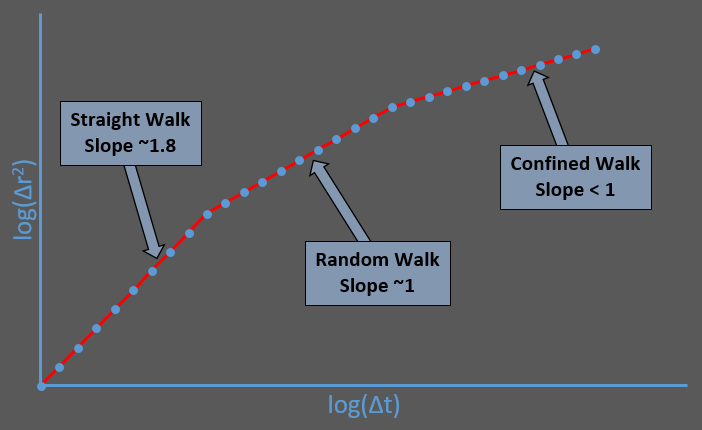
\includegraphics[width=0.6\linewidth]{log_diff.png}
%	\caption{Example investigation of live motion analysis using log-log plots.}
%	\label{fig:log-diff}
%\end{figure}
%
%\begin{itemize}
%\item In ecology, tracking data from tagged animals can be analyzed to find the roaming grounds of an animal.
%However, to distinguish random motion from the confined area to which an animal intentionally returns, we cannot simply look at the tracks by eye.
%A log-log plot can help us find the distances at which the motion gets confined; helping us determine the size of roaming grounds and how often roaming grounds are changed.
%In addition, on shorter timescales the motion will look directed since animals are able to move straight (at least over short distances)!
%\item On much smaller scales, within cells, the tracking data from individual molecules on a cell membrane have helped develop the theory of ``lipid rafts''. Such rafts are patches of membrane that float on the overall cell membrane. Within the raft sit a number of functional molecules that appear to operate together, taking advantage of their closeness to each other within a raft to enhance signals. The significance of lipid rafts in biology is still under investigation and log-log plots are a key tool to distinguish randomness from caged motion!
%\end{itemize}
%
%This particular choice is because when we make this choice, the function ex is its own derivative.
%That is, if we write $y = e^{x}$, then
%\[ \frac{dy}{dx} = y \text{.} \]
%\par
%In case you wondered how in the world a calculator figures out what ``$e$'' to the something is, the following result allows you to calculate the value of $e$ raised to some number -- eventually.
%\[ e^{x} = 1 + x + \frac{x^{2}}{2} + \frac{x^{3}}{6} + \frac{x^{4}}{24}+... \]
%You can see how this goes on - and it goes on forever.
%But for any fixed $x$ you are calculating for, the denominators go up faster than powers do, making the terms smaller and smaller so they can be dropped.
%\par 
%While this looks really messy and we're not going to use it, looking at it does give us two interesting messages.
%\begin{enumerate}
%\item \textbf{It explains why the exponential function is its own derivative.} If you take the derivative of the power series representation of the exponential, something interesting happens. The first term vanishes, the derivative of the linear term becomes the old first term (1), the derivative of the third (quadratic) term becomes the old second (linear) term, etc.  So the derivative of each term becomes the previous term in the original series.  We wind up getting the same thing back that we started with.  This also shows us why the denominators have the structure they do. [And with a little fancy mathematical footwork, we can show that the exponential is the only function that is its own derivative.]
%\item \textbf{It shows that we can only take exponentials of pure numbers.} Since we know that you can't add a length and an area - or any quantity that has units to its square - the power series only makes sense if ``x''  is a pure number.  You can't take an exponential of a quantity that has units.  Whenever in science we have an exponential, it will always be the ratio of two quantities with the same units - typically a variable and a scale for that variable.  (Like a time and a rate constant.)
%\end{enumerate}
%
%\section{Log-log Plots in Science}
%Log-Log plots have many uses in science.
%They are especially helpful for differentiating between different forms of \emph{functional dependency}.
%What is functional dependency? 
%Functional dependency tells us how one quantity varies when another is adjusted. 
%Example: for purely random motion, the diffusion of an object in 2-D space has a functional dependence like $\langle r^{2} \rangle = 4 D \Delta t$. 
%As you saw in lab, the viscosity and temperature of the fluid medium surrounding the object and the size of the object can affect the value of the diffusion constant, D, and thus the linear slope of the $\langle r^{2} \rangle$ vs.\ $\Delta t$ plot (where the slope is related to D). 
%A $log(\langle r^{2} \rangle)$ vs.\ $log(\Delta t)$ plot of this functional dependency would be a line with a slope of 1 — regardless of the value of the diffusion constant, D! 
%If we are not learning the diffusion constant D from this log-log plot, what does the slope of 1 tell us?
%\par 
%It turns out that the slope of $log(\langle r^{2} \rangle)$ vs.\ $log(\Delta t)$ tells us about what type of motion we are observing! 
%Most motion will not be linear in an $\langle r^{2} \rangle$ vs.\ $\Delta t$ plot. 
%There are other functional dependencies that can exist governing the relationship between $\langle r^{2} \rangle$ and $\Delta t$. 
%For directed motion at constant velocity, $\langle r^{2} \rangle$ changes as $(\Delta t)^{2}$ and so the $\langle r^{2} \rangle$ vs.\ $\Delta t$ plot would be quadratic. 
%But a $log(\langle r^{2} \rangle)$ vs.\ $log(\Delta t)$ plot of this motion is still linear, with a slope of 2. 
%For directed motion under uniform acceleration from rest, the distance traveled is $r = \frac{1}{2} a \Delta t^{2}$, so $\langle r^{2} \rangle$ changes linearly with $(\Delta t)^{4}$ — thus a $log(\langle r^{2} \rangle)$ vs.\ $log(\Delta t)$ plot of this motion has a slope of 4!
%\par 
%Other motion in cells is confined, e.g. molecules that are caged by a surrounding scaffolding of actin, or molecules on the membrane that are confined to a ``lipid raft'' or patch of membrane that has some functional activity. 
%For such caged motion, $\langle r^{2} \rangle$ does not quite increase linearly with $\Delta t$ — the distance moved gets smaller than we would expect for random motion as we get to larger and larger distances — thus a $log(\langle r^{2} \rangle)$ vs.\ $log(\Delta t)$ plot of this motion has a slope of less than 1.
% \par
%For real biological systems, the motion is often a combination of random and directed motion — and thus a $log(\langle r^{2} \rangle)$ vs.\ $log(\Delta t)$ plot of this motion has a slope between 1 and 2. 
%The dominant functional dependency (the one that determines the type of motion we observe) can also depend on the time scale at which we observe the motion.
%\par
%This is all very interesting, but how is it helpful to us?
%In biology, almost all motion can look quite random, but that apparently random motion can hide other processes that may look similar to random motion — in particular, caged motion:
%\begin{itemize}
%\item In ecology, tracking data from tagged animals can be analyzed to find the roaming grounds of an animal.
%However, to distinguish random motion from the confined area to which an animal intentionally returns, we cannot simply look at the tracks by eye.
%A log-log plot can help us find the distances at which the motion gets confined; helping us determine the size of roaming grounds and how often roaming grounds are changed.
%In addition, on shorter timescales the motion will look directed since animals are able to move straight (at least over short distances)!
%\item On much smaller scales, within cells, the tracking data from individual molecules on a cell membrane have helped develop the theory of ``lipid rafts''. Such rafts are patches of membrane that float on the overall cell membrane. Within the raft sit a number of functional molecules that appear to operate together, taking advantage of their closeness to each other within a raft to enhance signals. The significance of lipid rafts in biology is still under investigation and log-log plots are a key tool to distinguish randomness from caged motion!
%\end{itemize}
%%
%Below is a chart to help summarize the broad categories of functional dependency and their effects on the slope of the $log(\langle r^{2} \rangle)$ vs.\ $log(\Delta t)$ plots.
%
%
%\begin{table}[h!]
%	\centering
%	\begin{tabular}{|l|c|}
%	\hline 
%	Type of motion & Slope of the $log(\langle r^{2} \rangle)$ vs.\ $log(\Delta t)$ plot \\ 
%	\hline 
%	Confined & $s < 1$ \\ 
%	\hline 
%	Random & $s = 1$ \\ 
%	\hline 
%	Biological & $1 < s < 2$ \\ 
%	\hline 
%	Directed & $s = 2$ \\ 
%	\hline 
%	Accelerated & $s > 2$ \\ 
%	\hline 
%	\end{tabular} 
%	\caption{The effect of movement type on a log-log plot.}
%	\label{tab:logPlt}
%\end{table}
%These types of plots can also help us model a new phenomenon. 
%Imagine a situation in which you wish to develop a model of how a biological or chemical process spreads in space with increasing time. 
%Knowing the functional dependency between $\langle r^{2} \rangle$ and $\Delta t$ can help you build a model or help you choose between competing models. 
%Once we understand the model better, we can make predictions about what will happen when we make changes to the system. 
%In order to help us with our modeling, we take data on the motion and make a plot of $log(\langle r^{2} \rangle)$ vs.\ $log(\Delta t)$. 
%The slope of this plot helps us make decisions about what models to propose or what models to eliminate. 
%It also tells us which functional dependency dominates at which time scales — it tells us when a type of motion is the most important and when we can ignore the effects of other types of motion.
%\par
%(Note that log-log plots help with functional dependencies more generally. 
%In chemistry, you may need to plot the log of a molecule's solubility vs.\ the pH.
%Since the pH is the log of the number of free hydrogen ions, this is again a log-log plot in disguise! 
%Then the slope can tell you how many charges an atom or molecule has in solution.)
			%\ref{chap:log-plots}

\end{document}